\documentclass{article}


\usepackage{arxiv}

\usepackage[utf8]{inputenc} % allow utf-8 input
\usepackage[T1]{fontenc}    % use 8-bit T1 fonts
\usepackage{hyperref}       % hyperlinks
\usepackage{url}            % simple URL typesetting
\usepackage{booktabs}       % professional-quality tables
\usepackage{amsfonts}       % blackboard math symbols
\usepackage{nicefrac}       % compact symbols for 1/2, etc.
\usepackage{microtype}      % microtypography
\usepackage{lipsum}
\usepackage{graphicx}
\usepackage{float} 
\usepackage{subfigure}
\usepackage{appendix}
\usepackage{listings}
\usepackage{xcolor}
% \usepackage[hidelinks]{hyperref}

\title{AI-Addin \emph{Plugin for Interpretable Machine Learning}}


\author{
  Mengying Wang \\
  Computer System Engineering \\
  Northeastern University\\
  NUID: 001357559 \\
  \texttt{wang.mengyin@husky.neu.edu} \\
  %% examples of more authors
   \And
 Ruisi Gu \\
  Information System\\
  Northeastern University\\
  NUID: 001816641 \\
  \texttt{gu.ru@husky.neu.edu} \\
  %% \AND
  %% Coauthor \\
  %% Affiliation \\
  %% Address \\
  %% \texttt{email} \\
  %% \And
  %% Coauthor \\
  %% Affiliation \\
  %% Address \\
  %% \texttt{email} \\
  %% \And
  %% Coauthor \\
  %% Affiliation \\
  %% Address \\
  %% \texttt{email} \\
}

\begin{document}
\maketitle

\begin{abstract}
Despite widespread of automates analytical model building, most of the methods are black box models, which may lead to the situation that people hardly trust a machine learning prediction therefore not be able to make any change due to the result. However, the aim of utilizing machine learning method to predict a situation is to make some improvements and get a better result.

Our goal is to build a prototype which suitable for different types of datasets, this prototype is able to interpret models and data in a more understandable way. We provide several models to fit the dataset with the help of H2O libraries, including generalized linear model, logistic regression, decision tree and gradient boosting model. After model training, we demonstrate the interpretability by three different plots, they are variable importance, partial dependence plot and individual conditional expectation (ICE). Finally, we compare our model by matrix AUC and select the best model. Based on the interpretable plots from the best model, we are able to interpret the whole dataset. With the completion of prototype based on Amazon Reviews, we test this framework on a different dataset, Yelp Reviews, in order to validate the feasibility of prototype\cite{glm}.
\end{abstract}


% keywords can be removed
\keywords{Machine Learning Interpretability \and PDP \and ICE \and H2O}


\section{Introduction}
Machine Learning is rapidly growing area, new methods and research coming up every day. However, with machine learning continuously infiltrate into people’s lives, we have to deal with the problem that how to let people trust a machine learning prediction. Another problem we are facing is that how people could figure out a suitable method if all they can get from a machine learning model is a simple prediction. For example, if you go to a doctor for obesity, it’s hard to believe him if the doctor only gives you the conclusion that you will gain more weight. Beside the prove for this conclusion, you may also want to know the reason behind and also the method to prevent from gaining weight\cite{ml}.

On the aspect of training model, we take the advantage of H2O library and run the leaderboard of models which can fit the dataset best. Beside some advanced models such as GBM and XGBoost, we also train some basic models like GLM and Logistic Regression. These models may seem easy to train and use, but very useful and powerful regards fitting various types of datasets. Separating data into training and testing set would allow us to compare the models by calculating AUC scores. 

For model interpretability, we demonstrate our dataset in three different ways, which are variable importance, partial dependence plot and individual conditional expectation (ICE). Variable importance plot provides a list of the most significant variables in descending order by a mean decrease in Gini. The top variables contribute more to the model than the bottom ones and also have high predictive power in classifying default and non-default customers\cite{statistics}. A partial dependence plot can show whether the relationship between the target and a feature is linear, monotonous or more complex\cite{christoph}. Individual Conditional Expectation (ICE) plots display one line per instance that shows how the instance’s prediction changes when a feature changes\cite{christoph} \cite{plot}.

For each model, we generate three plots that mentioned above. Based on two matrixes, we select the best model and draw our conclusion by analyzing the plots we obtain. 



\section{Methods}
\label{sec:headings}


\subsection{Data Processing}
The tokenize function will split the reviews into words and remove any stop words, small words, or words with numbers in them. Then we group the vectors of similar words together in vector space by using Word2vec. Word2vec can make highly accurate guesses about a word’s meaning based on past appearances. Combining aggregated word embeddings columns with the original dataset.

\subsection{Training Models}
In order to get a general idea of our dataset within limit parameters and minimize processing runtime, we can take advantage of Auto ML in H2O. With the help of Auto ML, we are able to find the “best” model from building large number of models without any prior knowledge. H2O’s AutoML can be used for automating the machine learning workflow, which includes automatic training and tuning of many models within a user-specified time-limit\cite{AutoML}. 

\paragraph{Generalized Linear Model}
Since we already change our target into binomial class variable, we take family='binomial', model\_id='glm\_surrogate' as our first model. We use H2OGeneralizedLinearEstimator to initialize model and train the model based on our X (predictors), y (response) and training dataset. 
\paragraph{Logistic Regression}
For logistic regression model, we initialize by using model\_id="glm\_logistic" in H2OGeneralizedLinearEstimator. And based on the same X, y and training dataset.
\paragraph{GBM I}
In Gradient Boosting Model I, we generate the model based on hyperparameter as follow: ntrees=1, sample\_rate=1, col\_sample\_rate=1, max\_depth=3. However, model performance of GBM I is poor. That’s why we adjust our model hyperparameter and generate another GBM model, GBM II.
\paragraph{GBM II}
In Gradient Boosting Model II, instead of setting GBM hyperparameters ourselves, we use the model\_id="gbm.hex" initializing by H2OGradientBoostingEstimator. Beside that, we set some stop rules as below, stopping\_metric = "AUC", stopping\_tolerance = 0.001, stopping\_rounds = 5, score\_tree\_interval = 10.

\subsection{Model Interpretability}
In this section, we selected three basic Model-Agnostic Methods - Variable Importance or standardized coefficient plot, Partial Dependence Plot (PDP) and Individual Conditional Expectation (ICE) to make interpretability analysis for our model.

\paragraph{Variable Importance/ Standardized Coefficient}
which feature affect the predict results mostly deeply? 

This plot shows the top ten most important features in turn for the model. We called varimp\_plot() API of H2O to output a bar type plot  for them, the degree of importance is the length of the bar, the first one with a longest bar is the most important feature in this model, it means that predict results is deeply influenced by this feature, and the changing of this factor would result in the change of response variables.
\paragraph{Partial Dependence Plot (PDP)}
How the feature affect the predict results?

The partial dependence plot (short PDP or PD plot) shows the marginal effect one or two features have on the predicted outcome of a machine learning model\cite{pdp}. A mean status can be gotten in this plot, so it shows the general tendency between this feature and predict result.
\paragraph{Individual Conditional Expectation (ICE)}
How each instances affect the predict results?

The difference with the partial dependence plot (PDP) is that, the Individual Conditional Expectation (ICE) plots the tendency of every instance, so that we can get the difference between different instances and the scope of all instances. ecause H2o doesn’t have the package to plot it, so we use the package PyCEbox for panda’s dataframe, and convert it to suit for our h2o Frame.
In order to apply ICE plot under H2O environment, we disassembled the package in pandas and convert into H2O version, then save it into a py file which is easy to refer. View the code in Appendix \ref{sec:App}. 
\section{Results}

\subsection{Leaderboard}
Figure \ref{Fig.leaderboard_a} and Figure \ref{Fig.leaderboard_y} are the output of H2O’s AutoML, it can be used for automating the machine learning workflow, which includes automatic training and tuning of many models within a user-specified time-limit. With the help of Auto ML LeaderBoard, we are able to find the “best” model from building large number of models without any prior knowledge\cite{AutoML}.

\begin{figure}[ht]
\centering
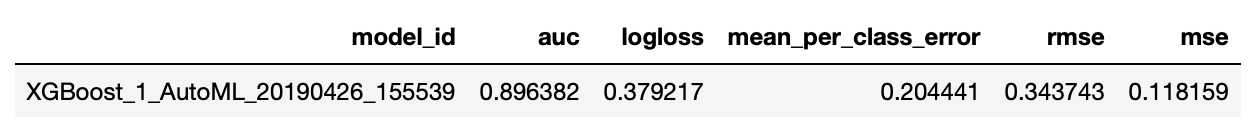
\includegraphics[scale=0.6]{plots/amazon/leaderboard.png}
\caption{leaderboard of Prototype dataset}
\label{Fig.leaderboard_a}
\end{figure}

\begin{figure}[ht]
\centering
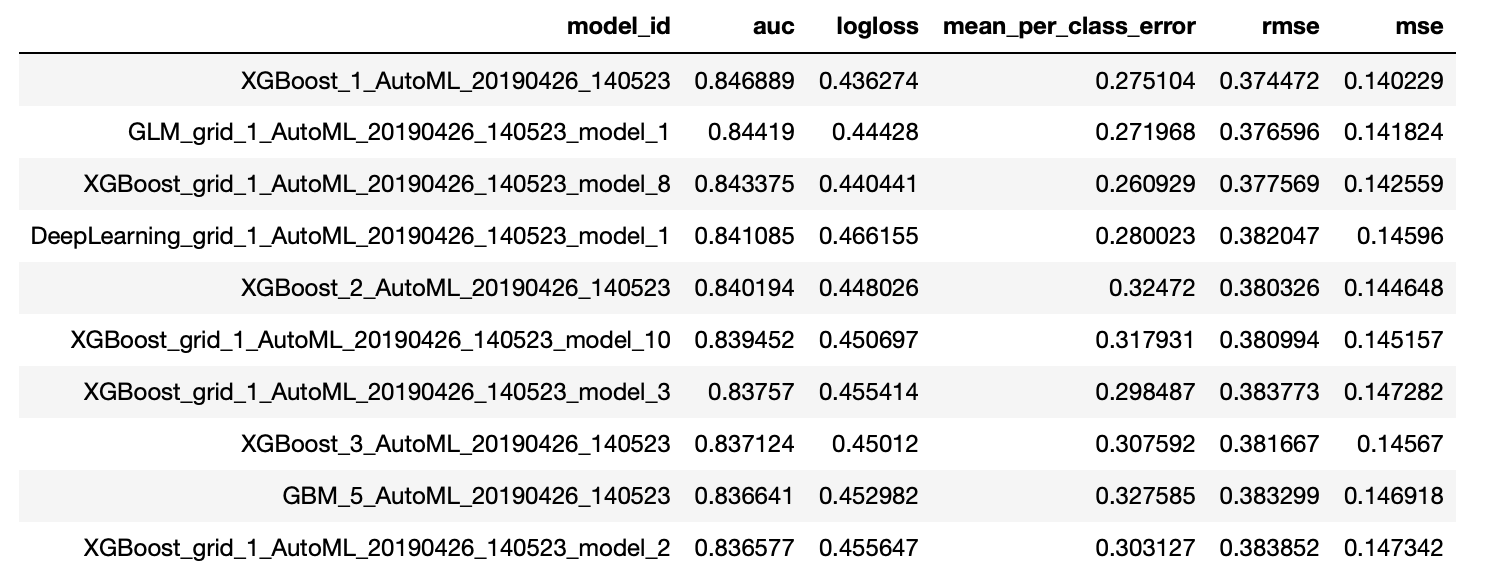
\includegraphics[scale=0.6]{plots/yelp/leaderboard.png}
\caption{leaderboard of testing dataset}
\label{Fig.leaderboard_y}
\end{figure}


\subsection{Prototype}


\subsubsection{Variable Importance/ Standardized Coefficient}
Figure \ref{Fig.a.v} has four sub figures for different models' variable importance or standardized coefficient plots in Amazon Review. For each plot, the first one with the longest bar is the most important feature in its model. So we can get that, for Generalized Linear Model, "HelpfulnessNumerator" is the most important, in the same way, C2 for Logistic Regression, Summary\_C91 for Gradient Boosting Model I and C45 for Gradient Boosting Model II.

\begin{figure}[H]
\centering
\subfigure[Generalized Linear]{
\begin{minipage}[t]{0.48\textwidth}
\centering
\label{Fig.a.v.1}
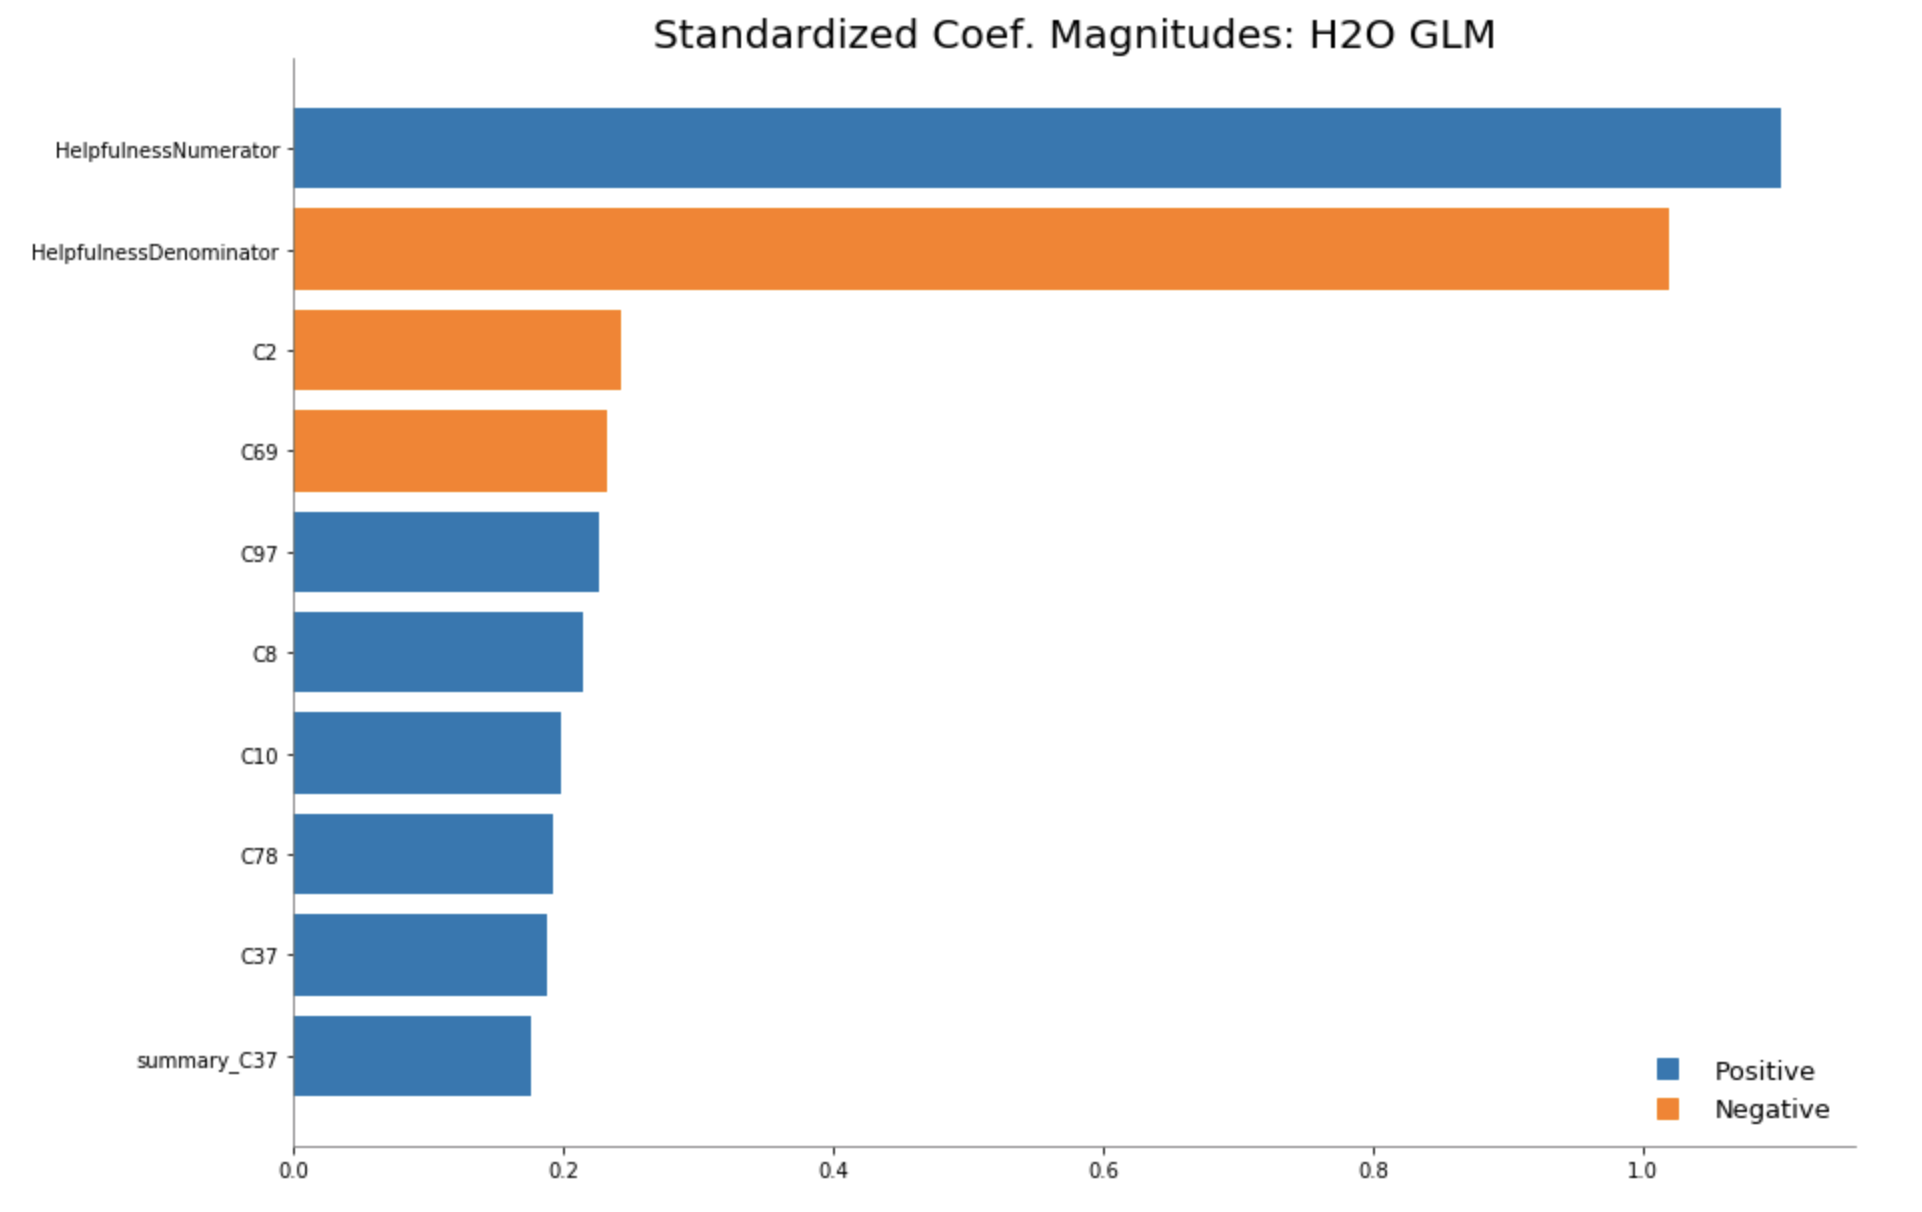
\includegraphics[width=6cm]{plots/amazon/a_vi_glm.png}
\end{minipage}
}
\subfigure[Logistic Regression]{
\begin{minipage}[t]{0.48\textwidth}
\centering
\label{Fig.a.v.2}
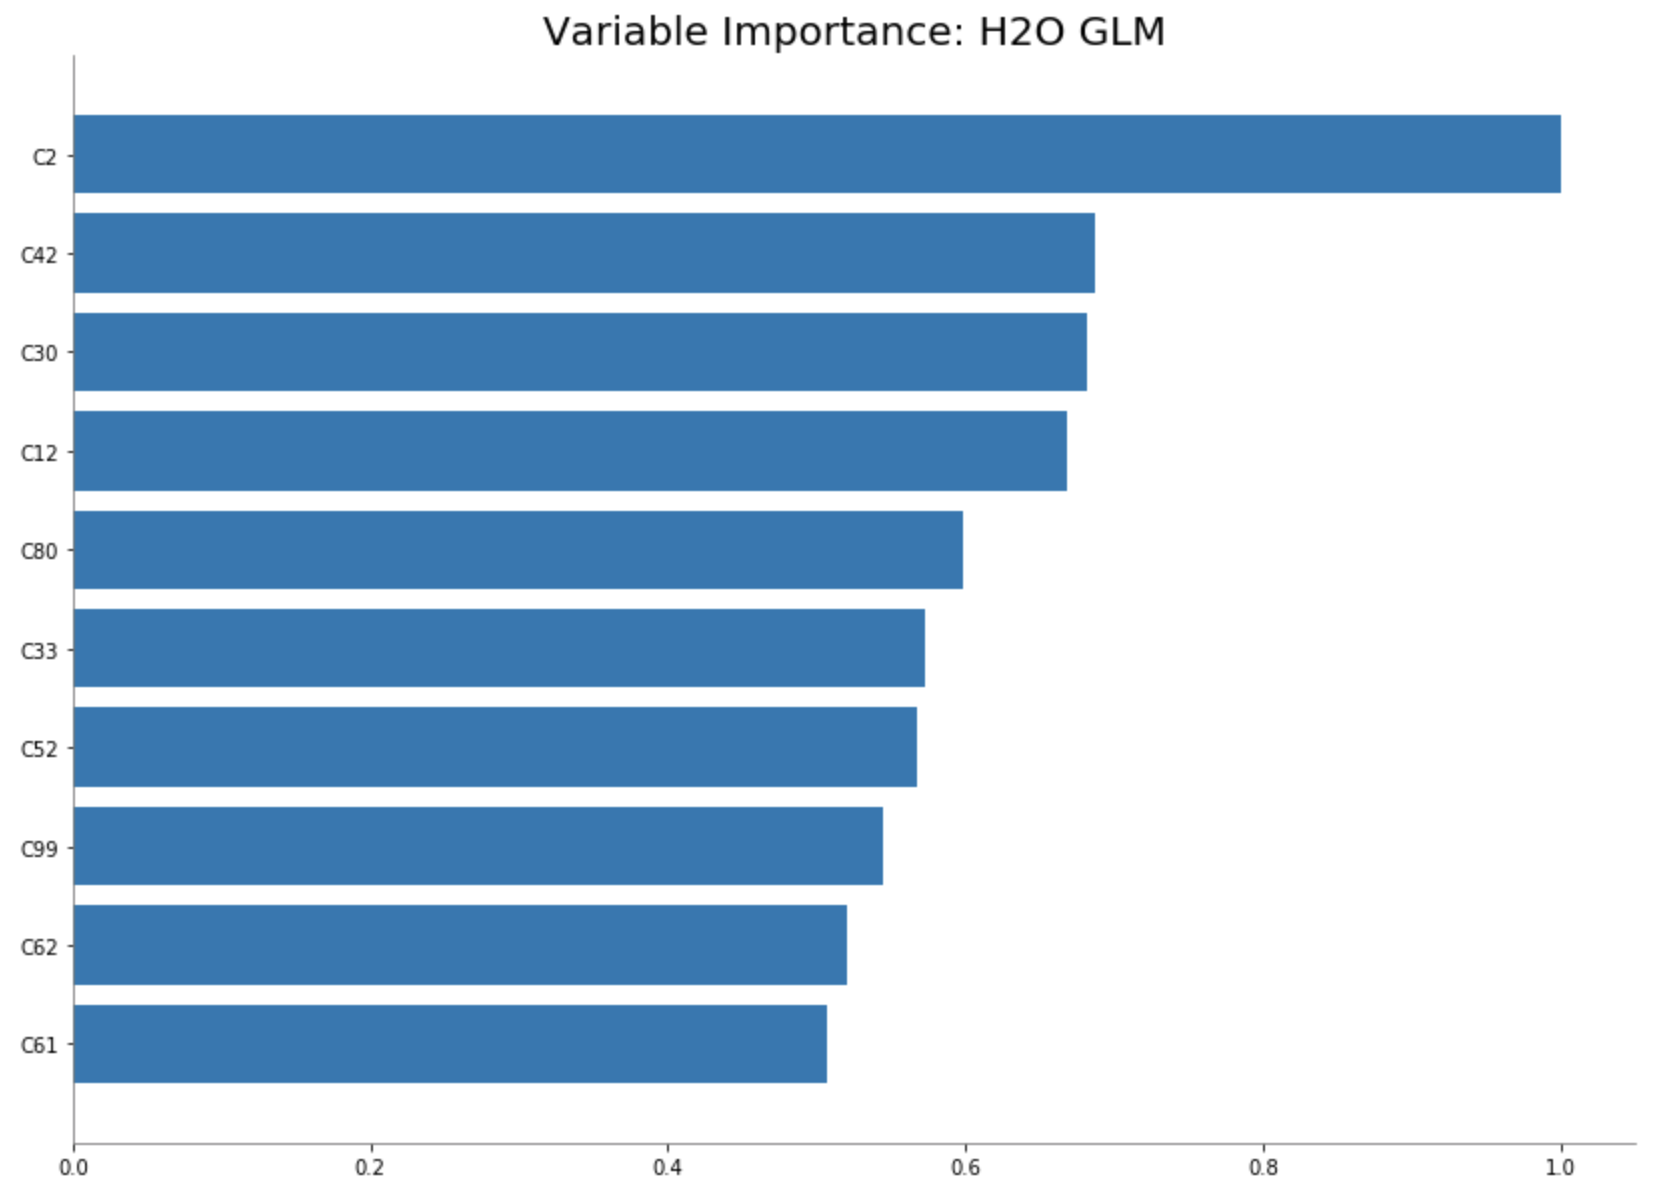
\includegraphics[width=6cm]{plots/amazon/a_vi_lr.png}
\end{minipage}
}
\quad
\subfigure[Gradient Boosting I]{
\begin{minipage}[t]{0.48\textwidth}
\centering
\label{Fig.a.v.3}
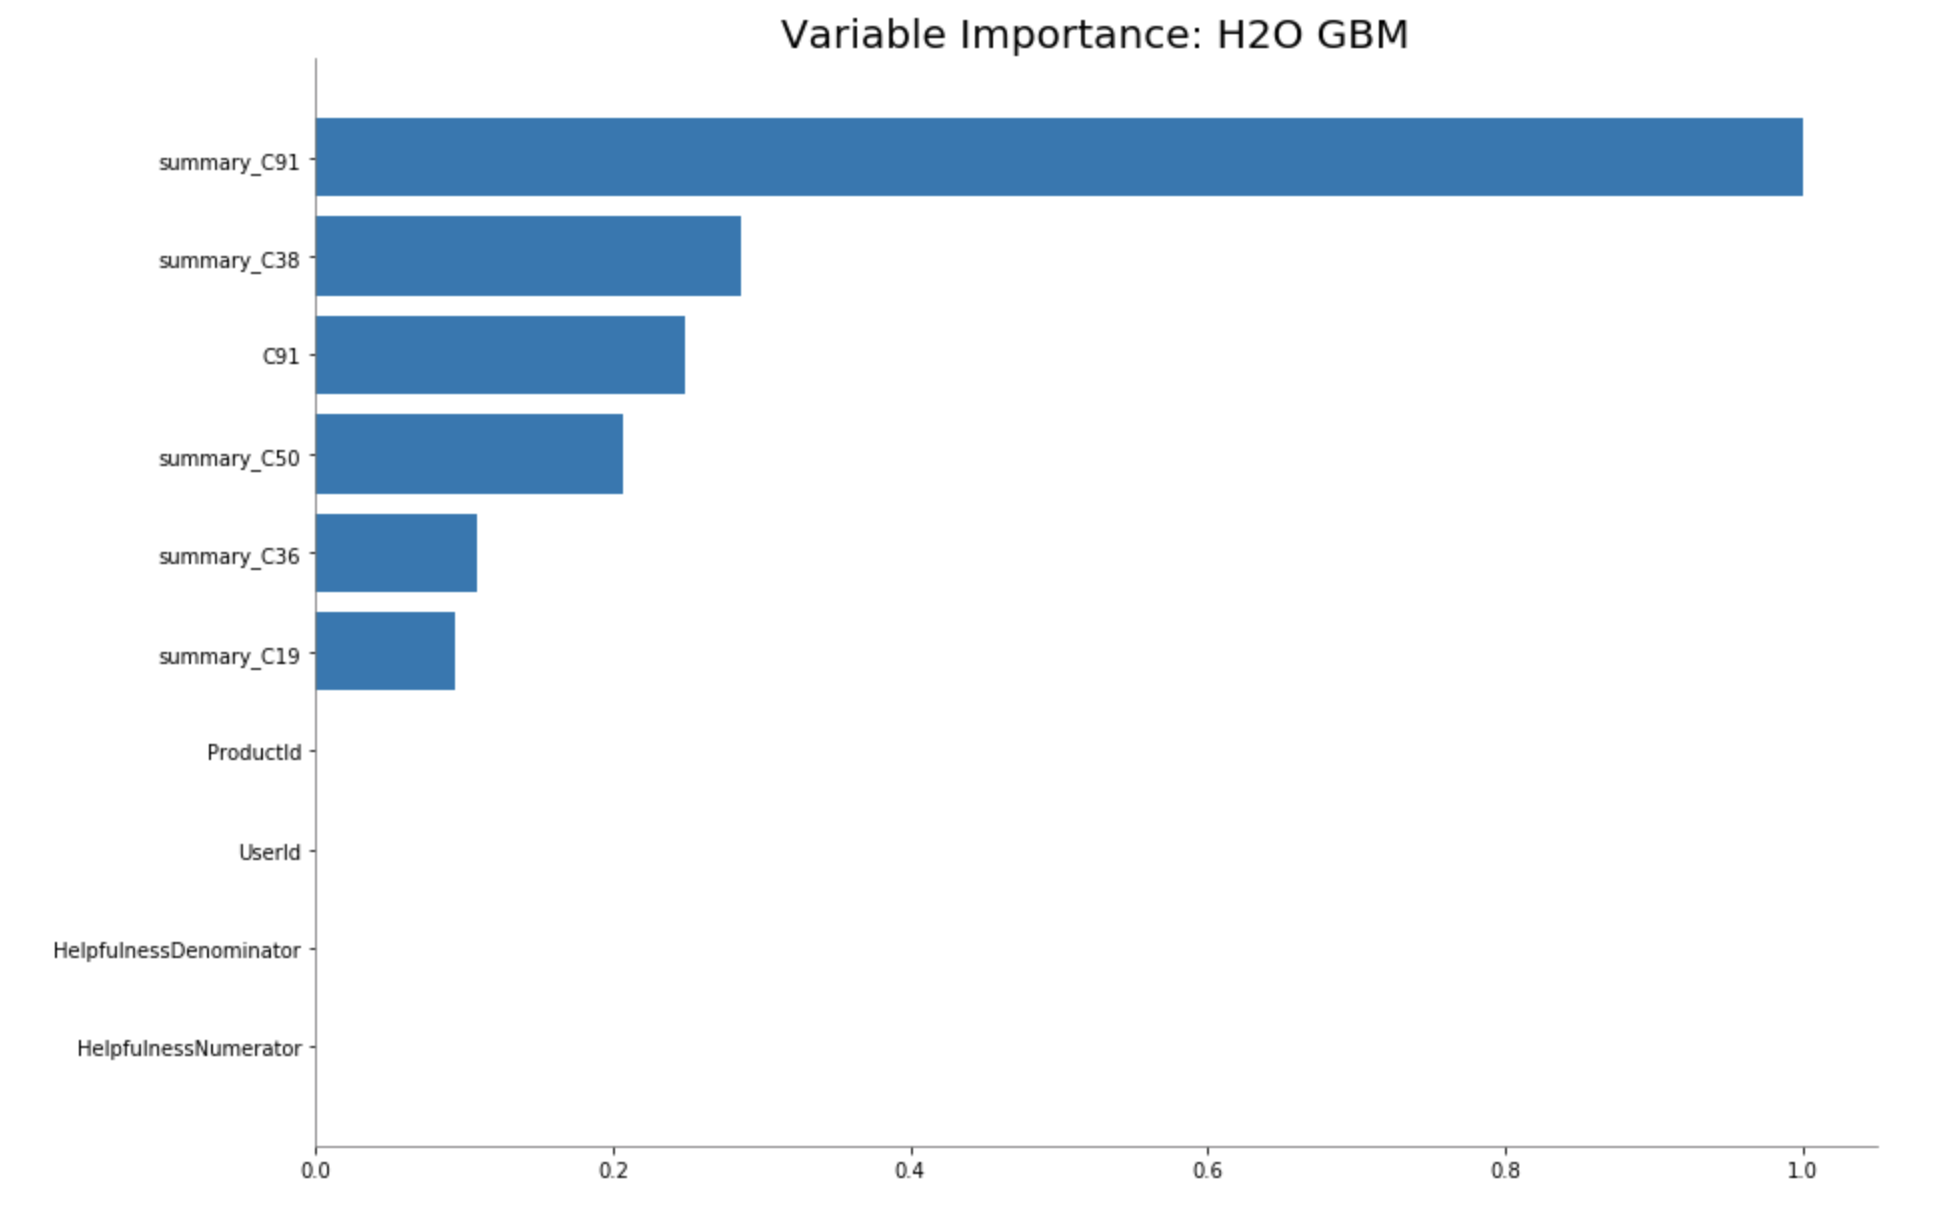
\includegraphics[width=6cm]{plots/amazon/a_vi_gbm1.png}
\end{minipage}
}
\subfigure[Gradient Boosting II]{
\begin{minipage}[t]{0.48\textwidth}
\centering
\label{Fig.a.v.4}
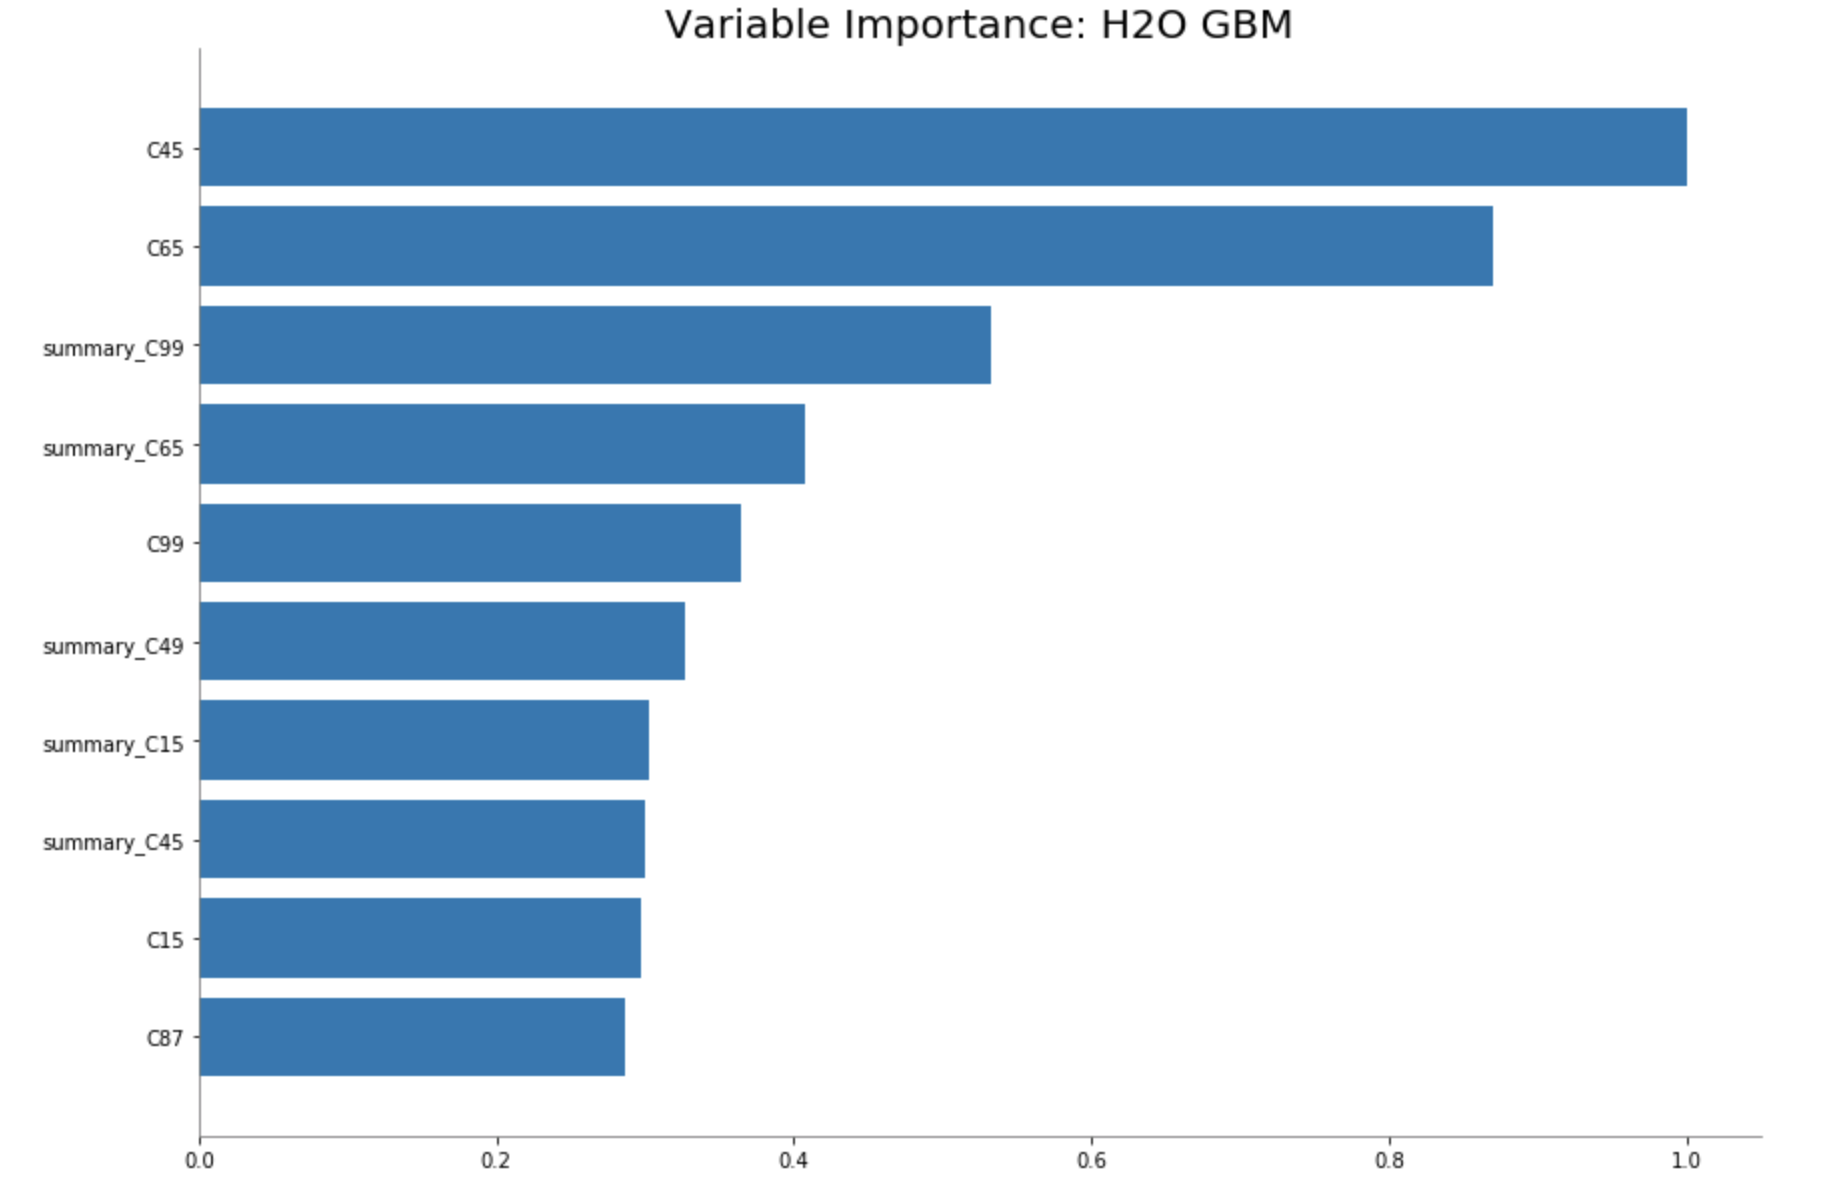
\includegraphics[width=6cm]{plots/amazon/a_vi_gbm2.png}
\end{minipage}
}
\caption{Variable Importance/ Standardized Coefficient Plots for Amazon Reviews}
\label{Fig.a.v}
\end{figure}


\subsubsection{Partial Dependence Plot}
Figure \ref{Fig.a.p} has four sub figures for different models' Partial Dependence Plots (PDP) in Amazon Review. We use the most important feature which we got in Figure \ref{Fig.a.v} as x axis, and the mean of Positive Review is the y axis. In Generalized Linear Model, We can get that the positive reviews always have a "HelpfulnessNumerator" larger than 100, and in Logistic Regression, the larger the C2 is, the less probability to get a positive review. In the last two Gradient Boosting Models, the mean of Positive Review change smoothly with the change of important features summary\_C91 and C45.

\begin{figure}[H]
\centering
\subfigure[Generalized Linear]{
\begin{minipage}[t]{0.48\textwidth}
\centering
\label{Fig.a.p.1}
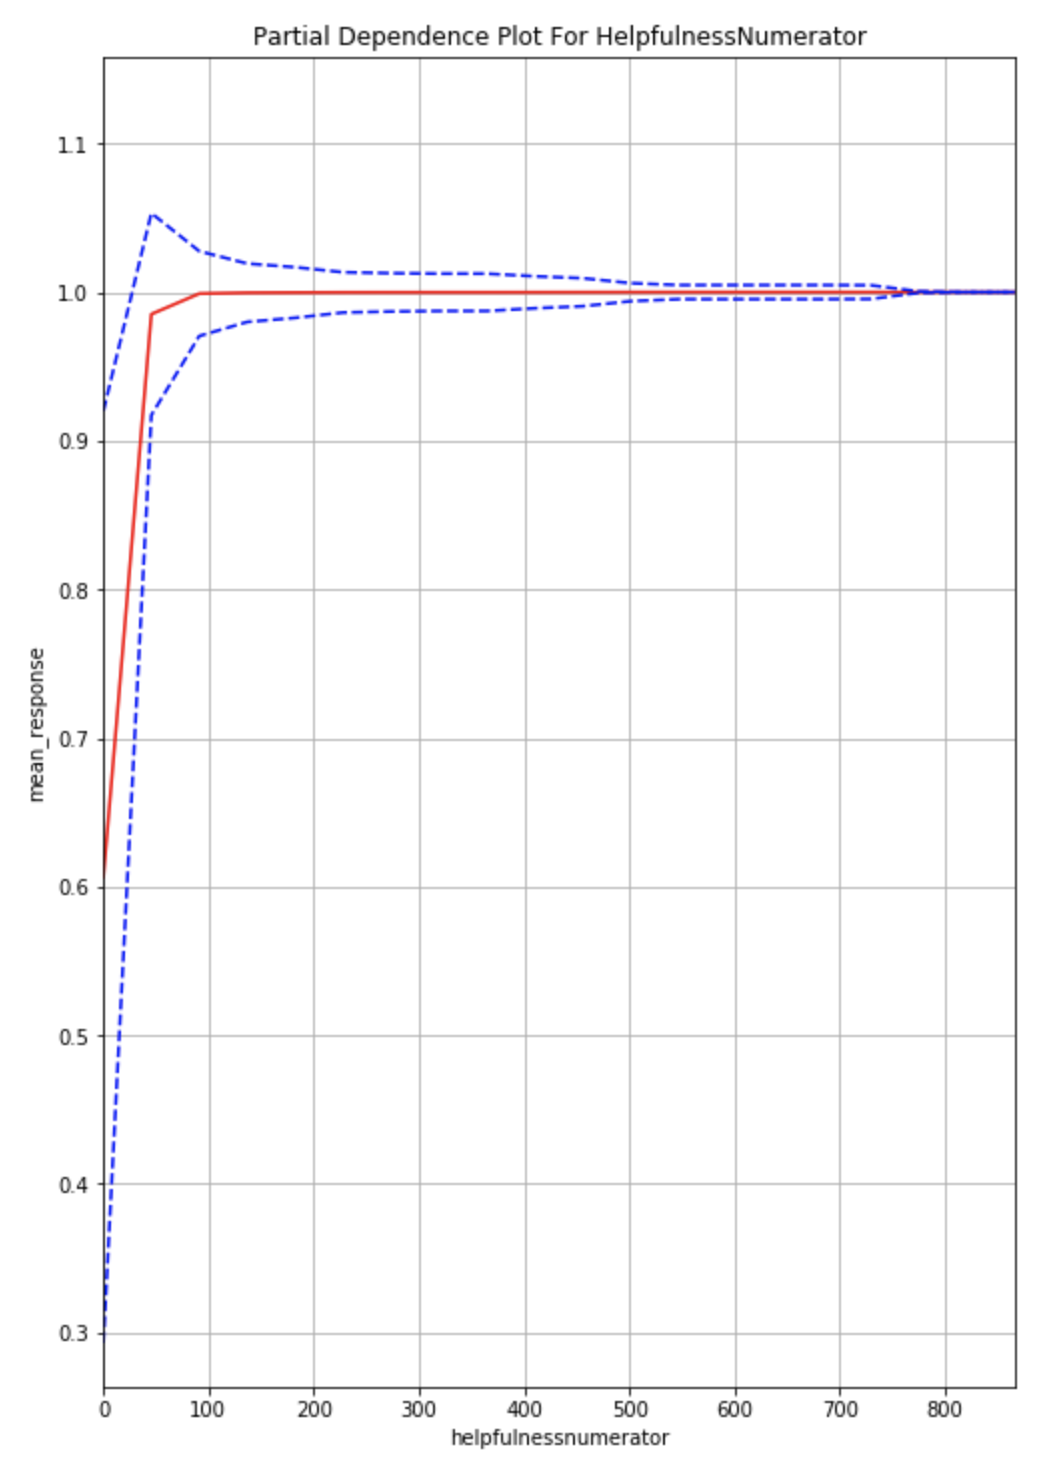
\includegraphics[width=6cm]{plots/amazon/a_pdp_glm.png}
\end{minipage}
}
\subfigure[Logistic Regression]{
\begin{minipage}[t]{0.48\textwidth}
\centering
\label{Fig.a.p.2}
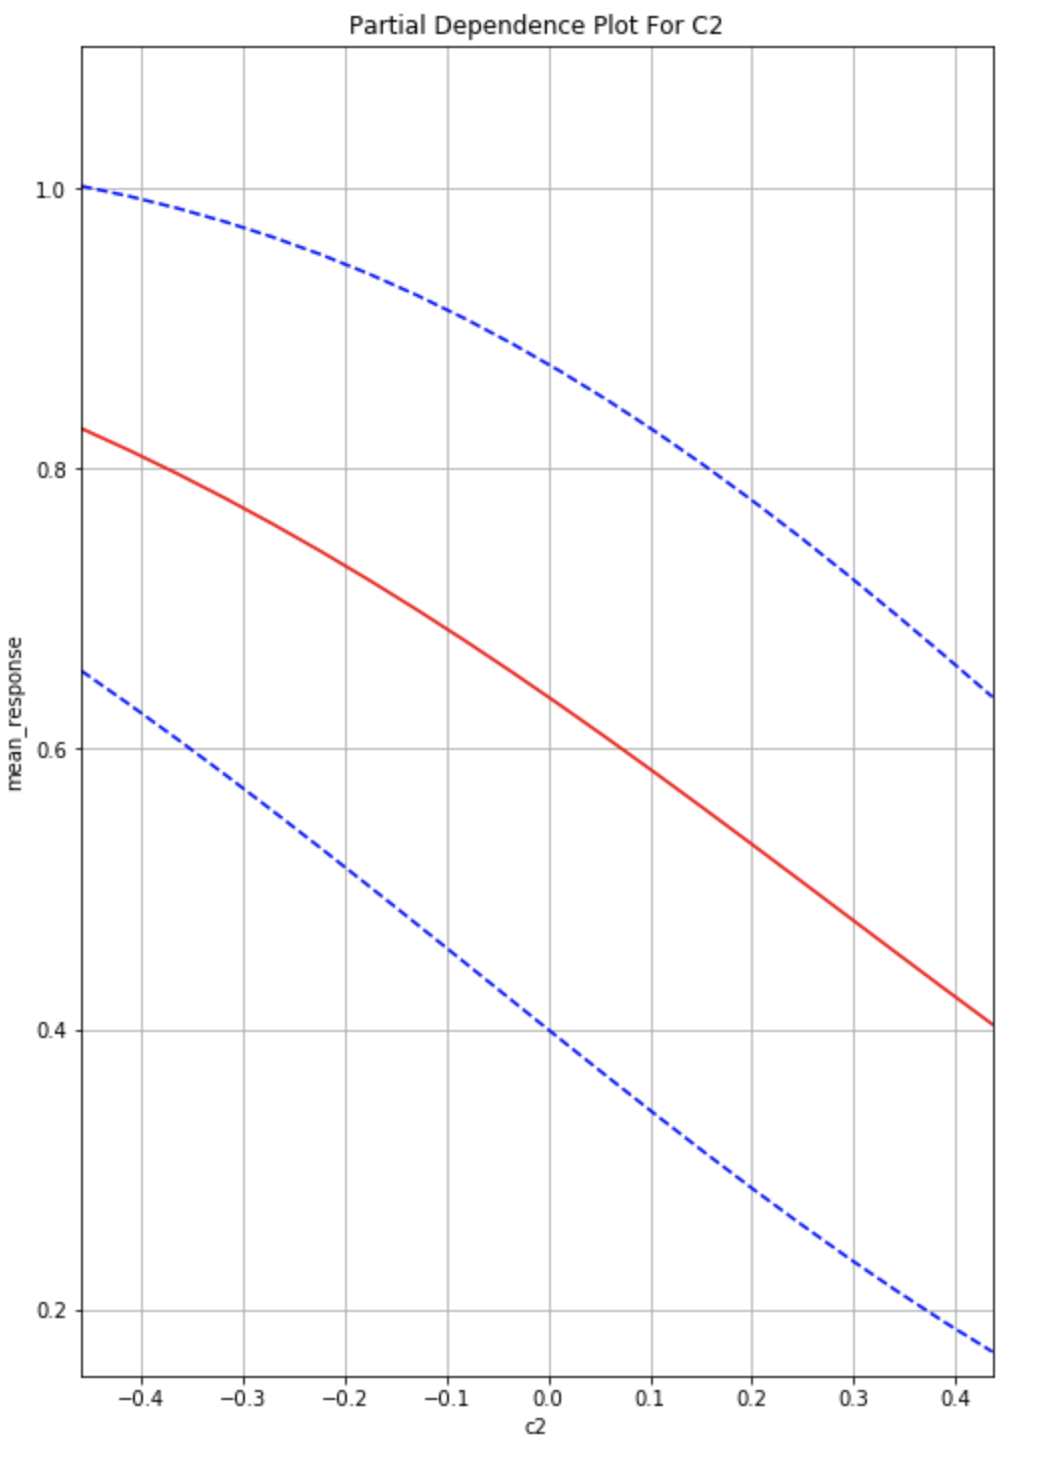
\includegraphics[width=6cm]{plots/amazon/a_pdp_lr.png}
\end{minipage}
}
\end{figure}
\addtocounter{figure}{-1}   
\begin{figure} 
\addtocounter{figure}{1}      
\centering 
\subfigure[Gradient Boosting I]{
\begin{minipage}[t]{0.48\textwidth}
\centering
\label{Fig.a.p.3}
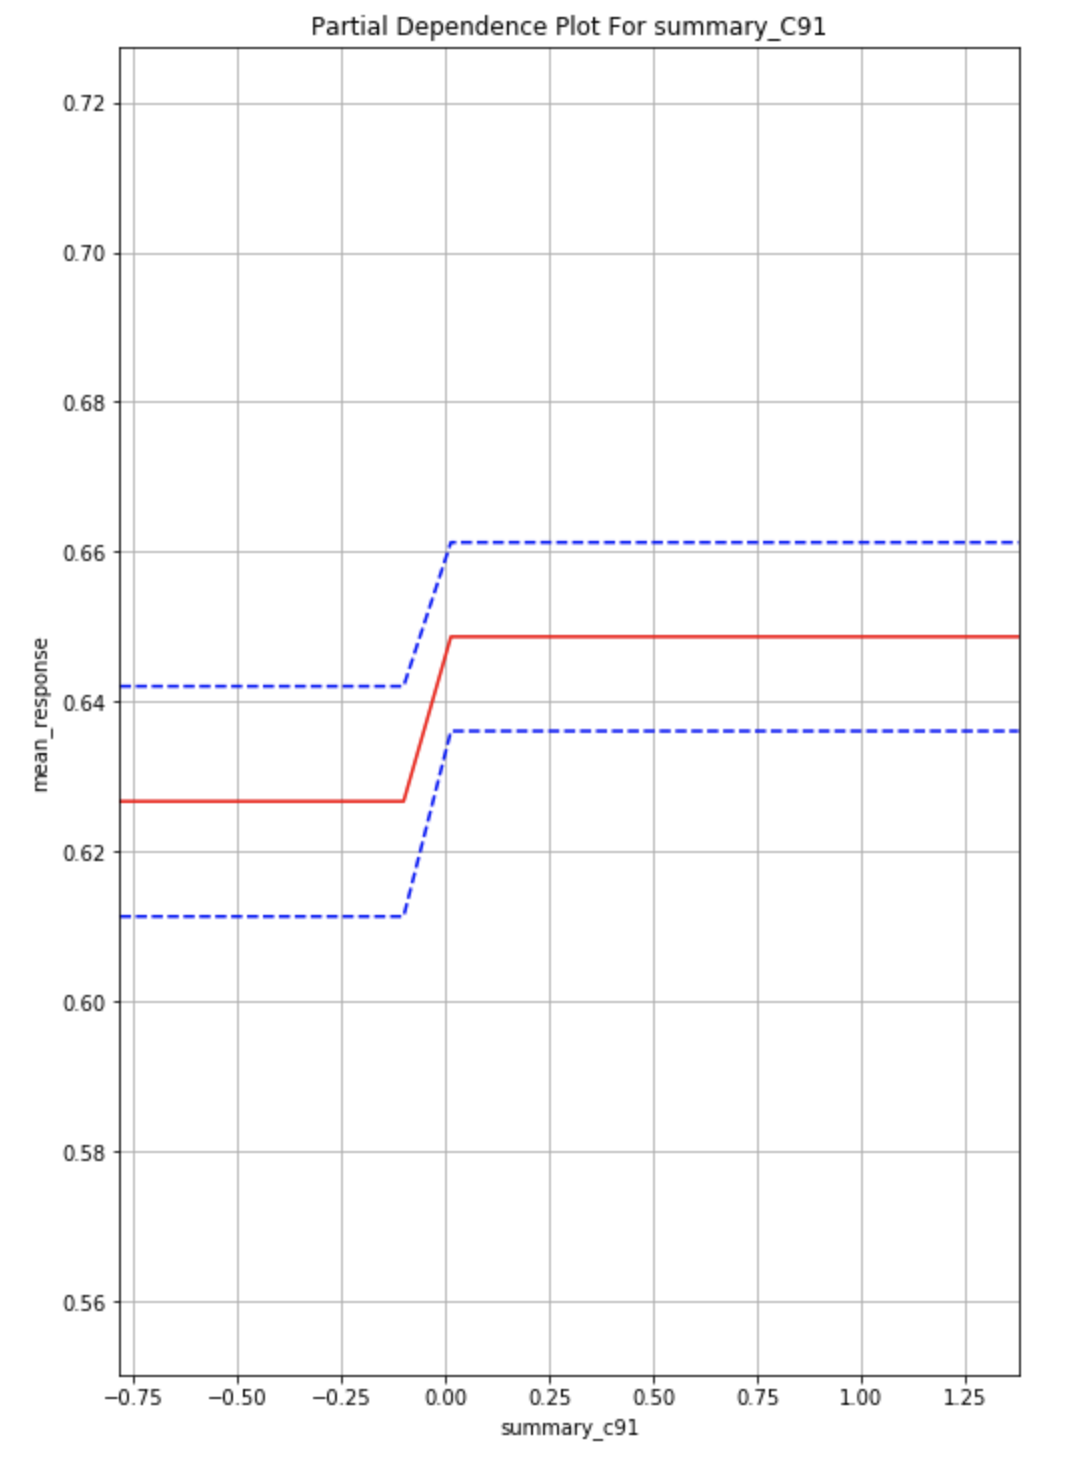
\includegraphics[width=6.2cm]{plots/amazon/a_pdp_gbm1.png}
\end{minipage}
}
\subfigure[Gradient Boosting II]{
\begin{minipage}[t]{0.48\textwidth}
\centering
\label{Fig.a.p.4}
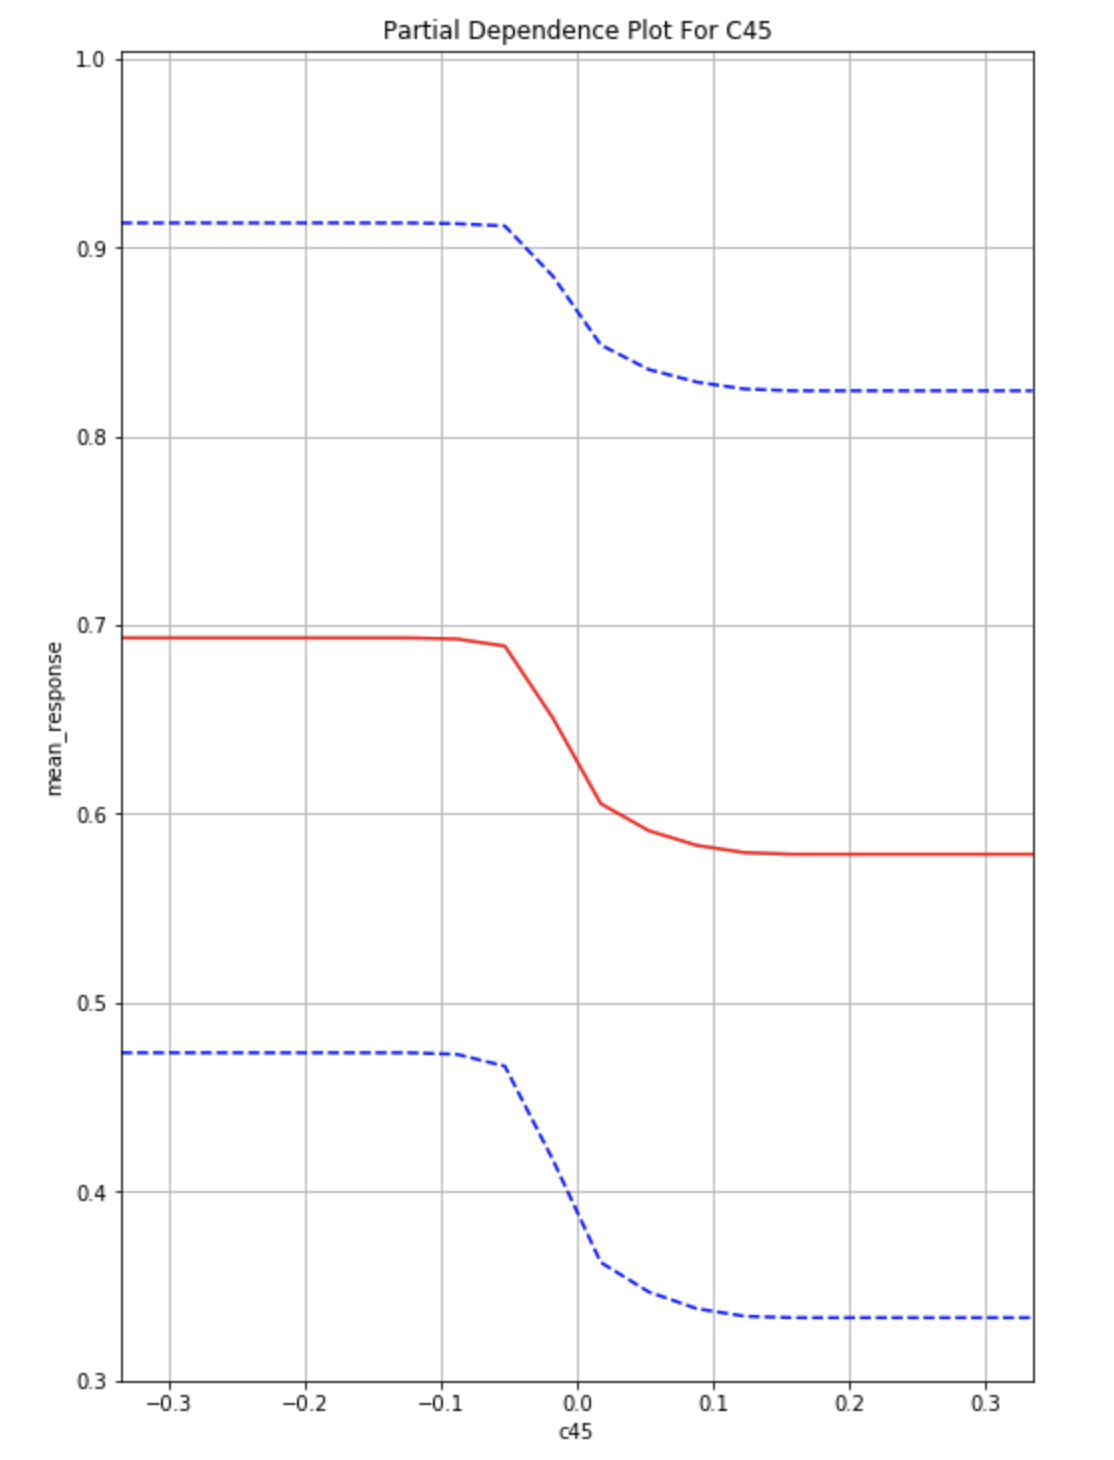
\includegraphics[width=6.2cm]{plots/amazon/a_pdp_gbm2.png}
\end{minipage}
}
\caption{Partial Dependence Plots (PDP) for Amazon Reviews}
\label{Fig.a.p}
\end{figure}



\subsubsection{Individual Conditional Expectation}
Figure \ref{Fig.a.i} has four sub figures for different models' Individual Conditional Expectation (ICE) in Amazon Review. Base on all these four plots, the instances in Figure \ref{Fig.a.i.1}, Figure \ref{Fig.a.i.2} and Figure \ref{Fig.a.i.3}, especially the Logistic Regression. On the contrary, the instances in are \ref{Fig.a.i.3} focused in a small range. We also can get that the general tendency of ICE change accords with PDP in Figure \ref{Fig.a.p} above.

\begin{figure}[H]
\centering
\subfigure[Generalized Linear]{
\begin{minipage}[t]{0.48\textwidth}
\centering
\label{Fig.a.i.1}
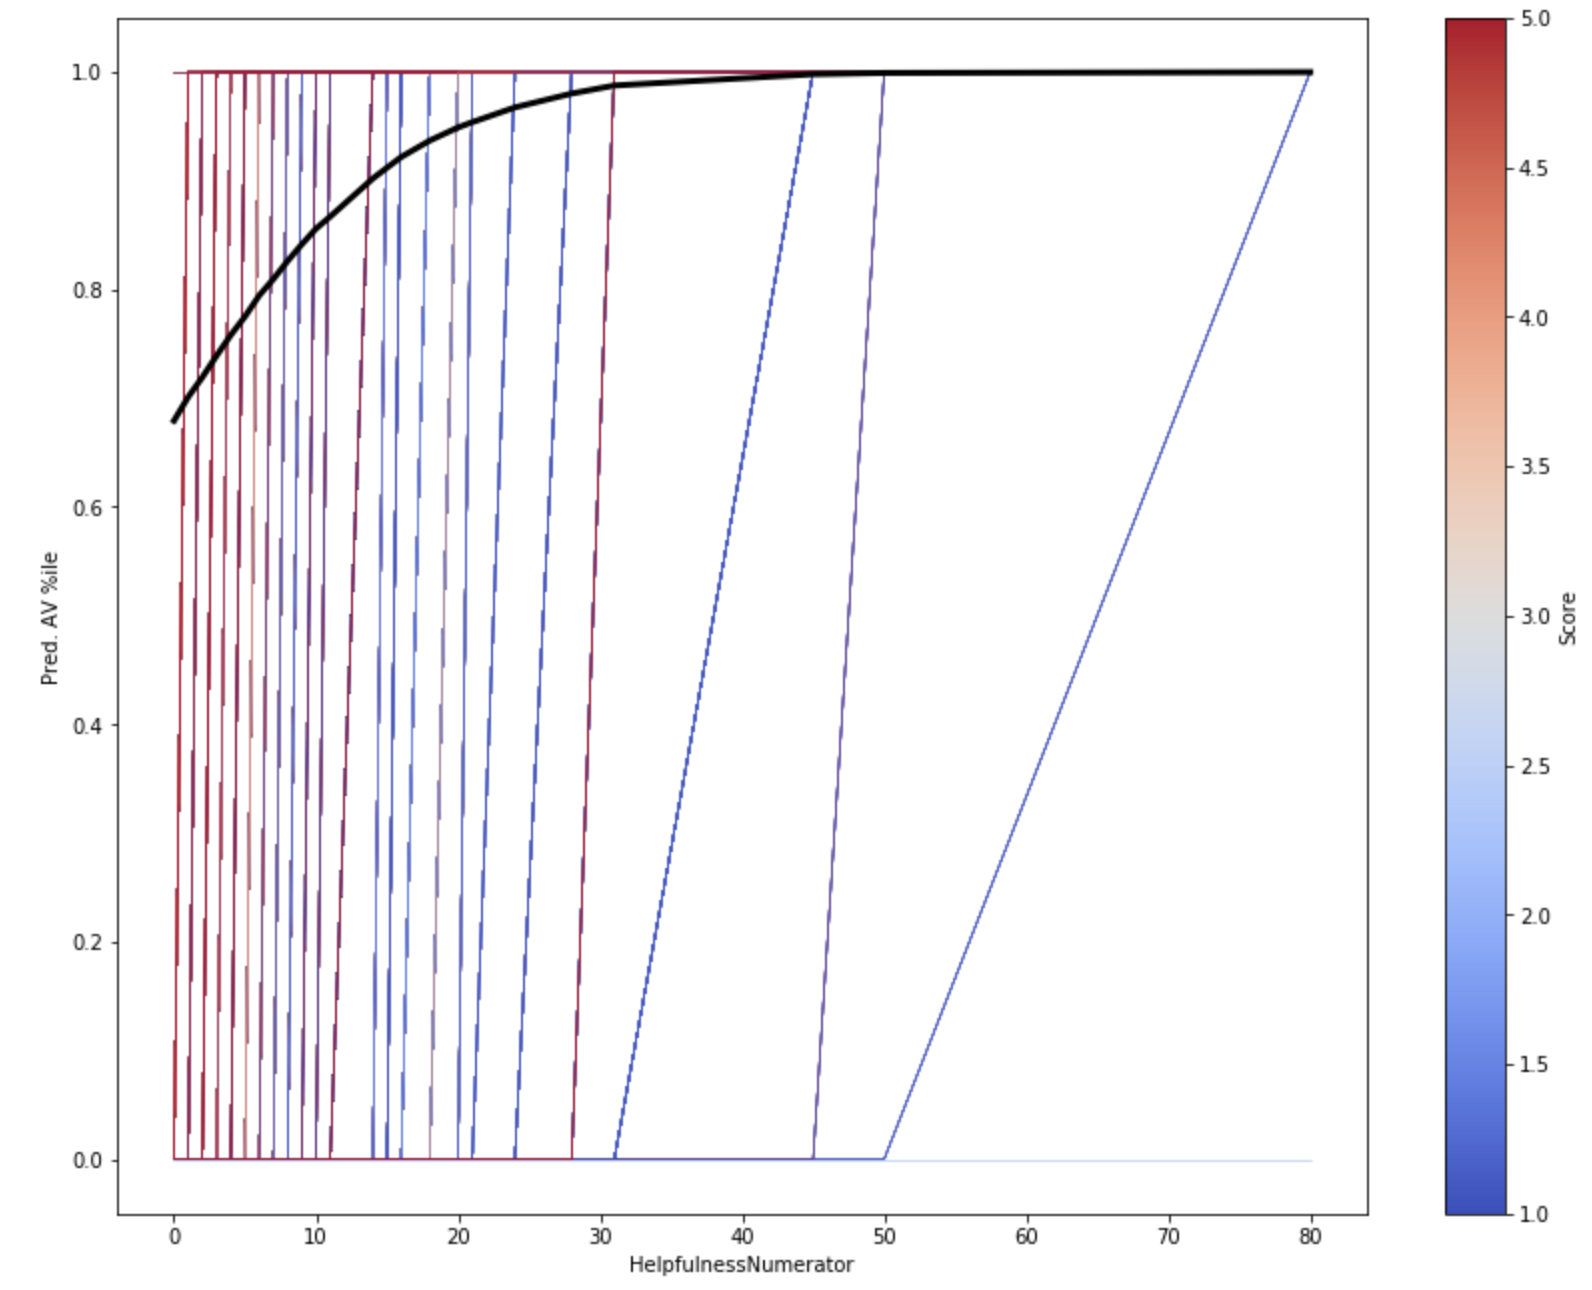
\includegraphics[width=6cm]{plots/amazon/a_ice_glm.png}
\end{minipage}
}
\subfigure[Logistic Regression]{
\begin{minipage}[t]{0.48\textwidth}
\centering
\label{Fig.a.i.2}
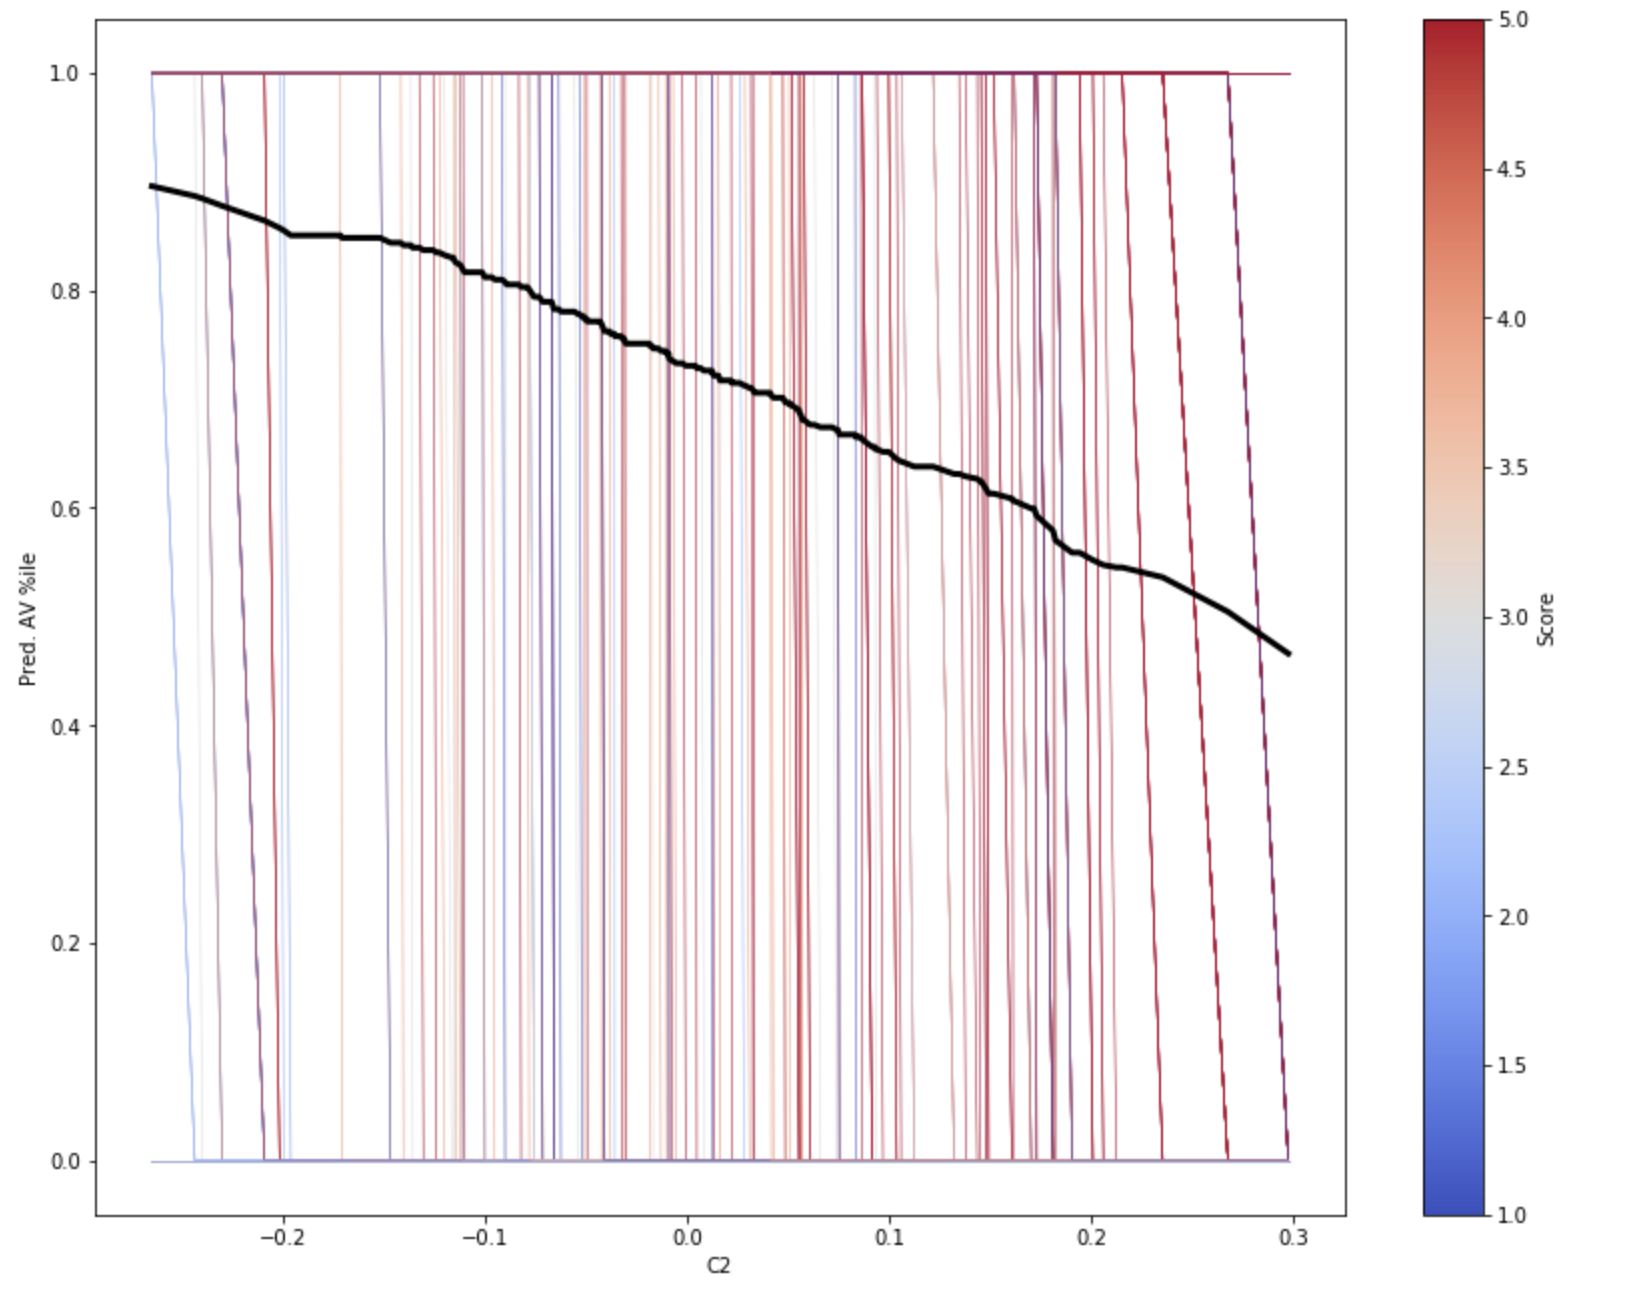
\includegraphics[width=6cm]{plots/amazon/a_ice_lr.png}
\end{minipage}
}
\end{figure}
\addtocounter{figure}{-1}   
\begin{figure} [H]
\addtocounter{figure}{1}      
\centering
\subfigure[Gradient Boosting I]{
\begin{minipage}[t]{0.48\textwidth}
\centering
\label{Fig.a.i.3}
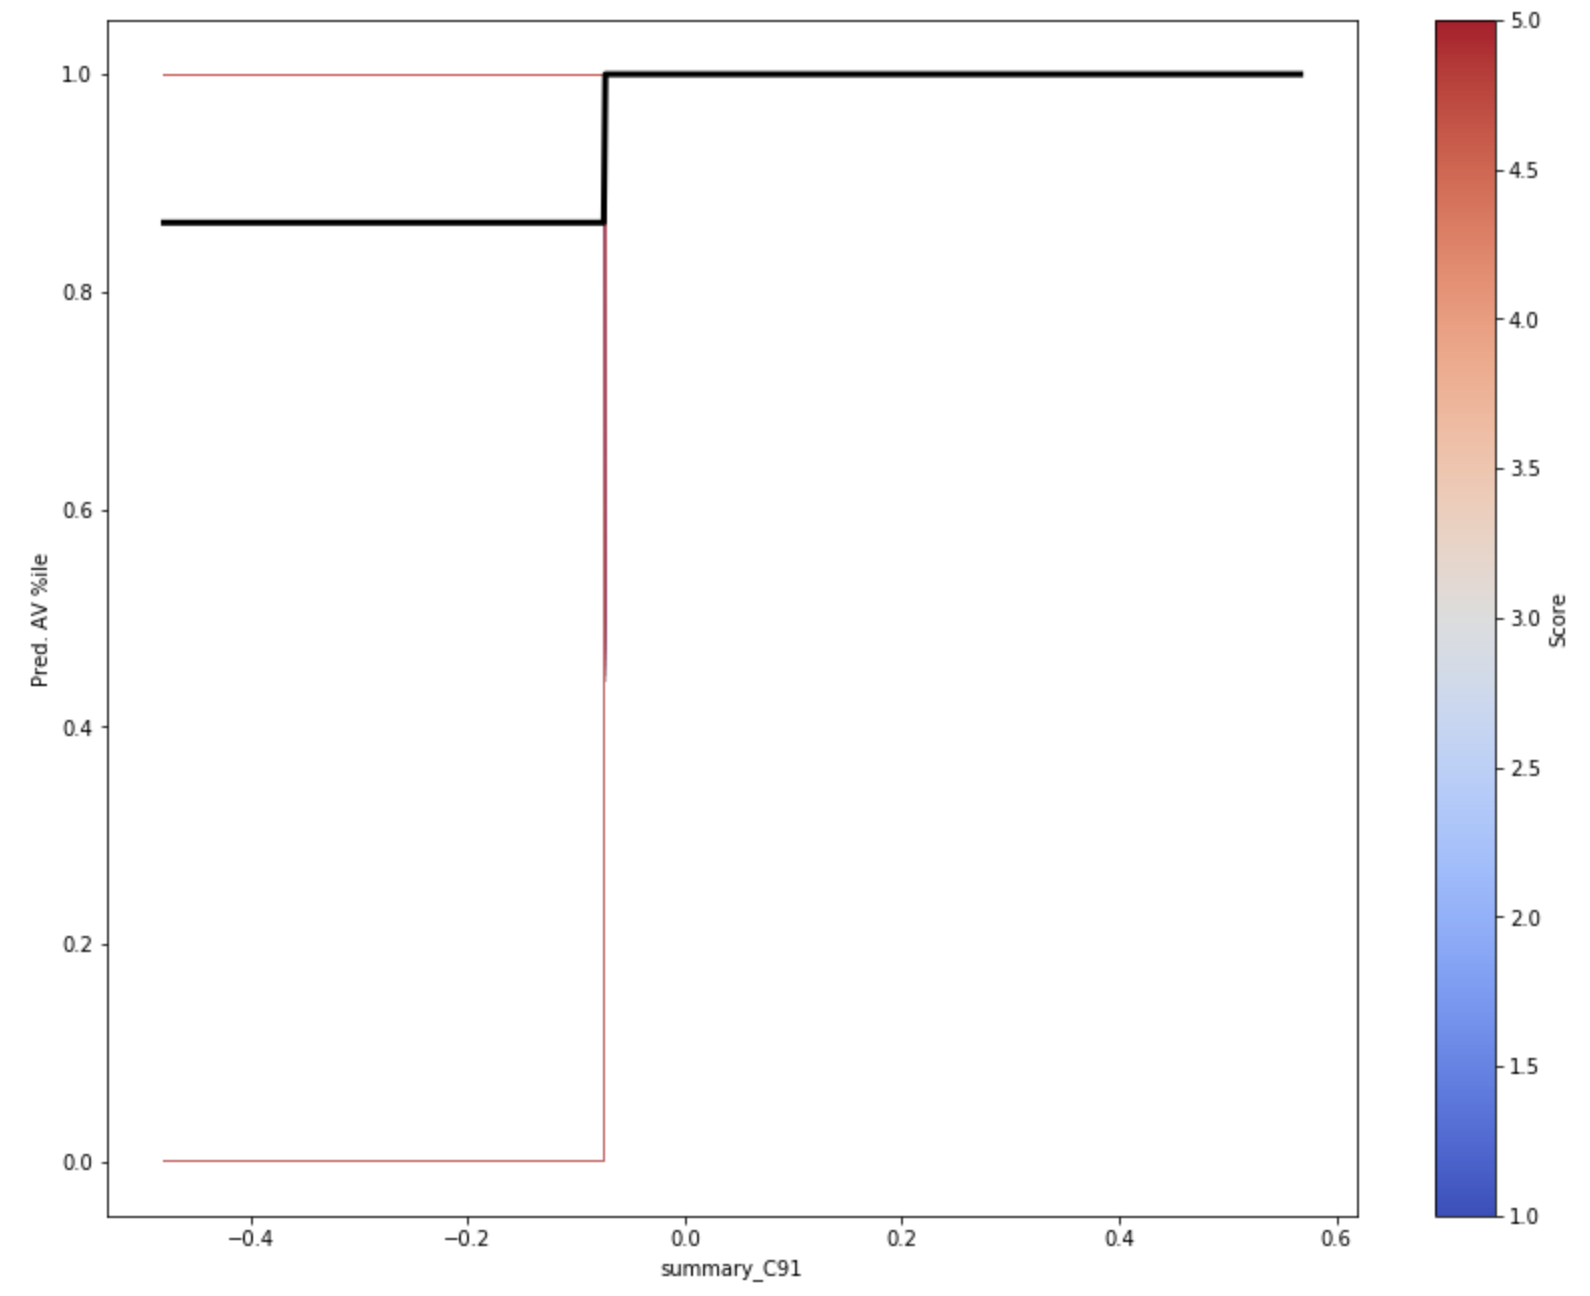
\includegraphics[width=6cm]{plots/amazon/a_ice_gbm1.png}
\end{minipage}
}
\subfigure[Gradient Boosting II]{
\begin{minipage}[t]{0.48\textwidth}
\centering
\label{Fig.a.i.4}
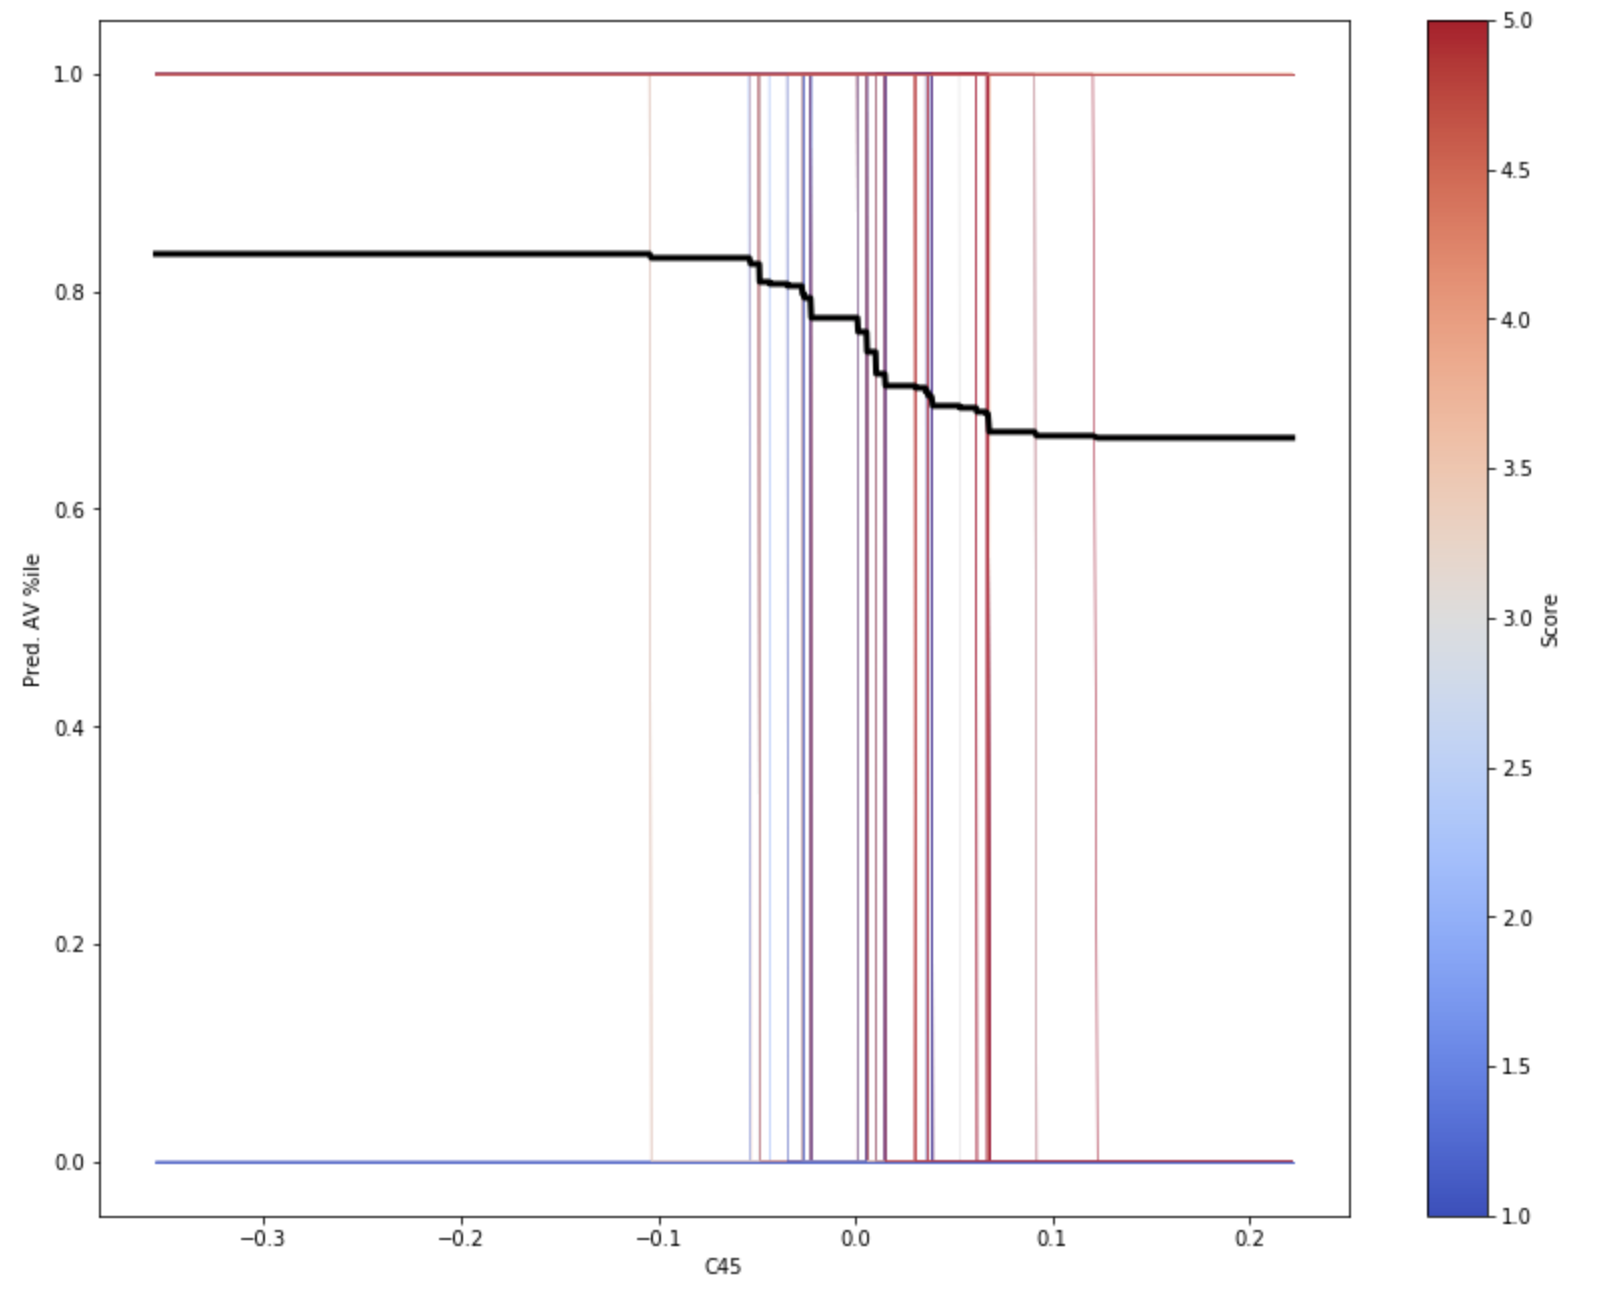
\includegraphics[width=6cm]{plots/amazon/a_ice_gbm2.png}
\end{minipage}
}
\caption{Individual Conditional Expectation (ICE) for Yelp Reviews}
\label{Fig.a.i}
\end{figure}

\subsection{Test on new dataset}

\subsubsection{Variable Importance/ Standardized Coefficient}
Figure \ref{Fig.y.v} has four sub figures for different models' variable importance or standardized coefficient plots in Yelp Review. We can get that, for Generalized Linear Model, "user\_id" is the most important, in the same way, C40 for Logistic Regression, C2 for Gradient Boosting Model I and Gradient Boosting Model II.
\begin{figure}[H]
\centering
\subfigure[Generalized Linear]{
\begin{minipage}[t]{0.48\textwidth}
\centering
\label{Fig.y.v.1}
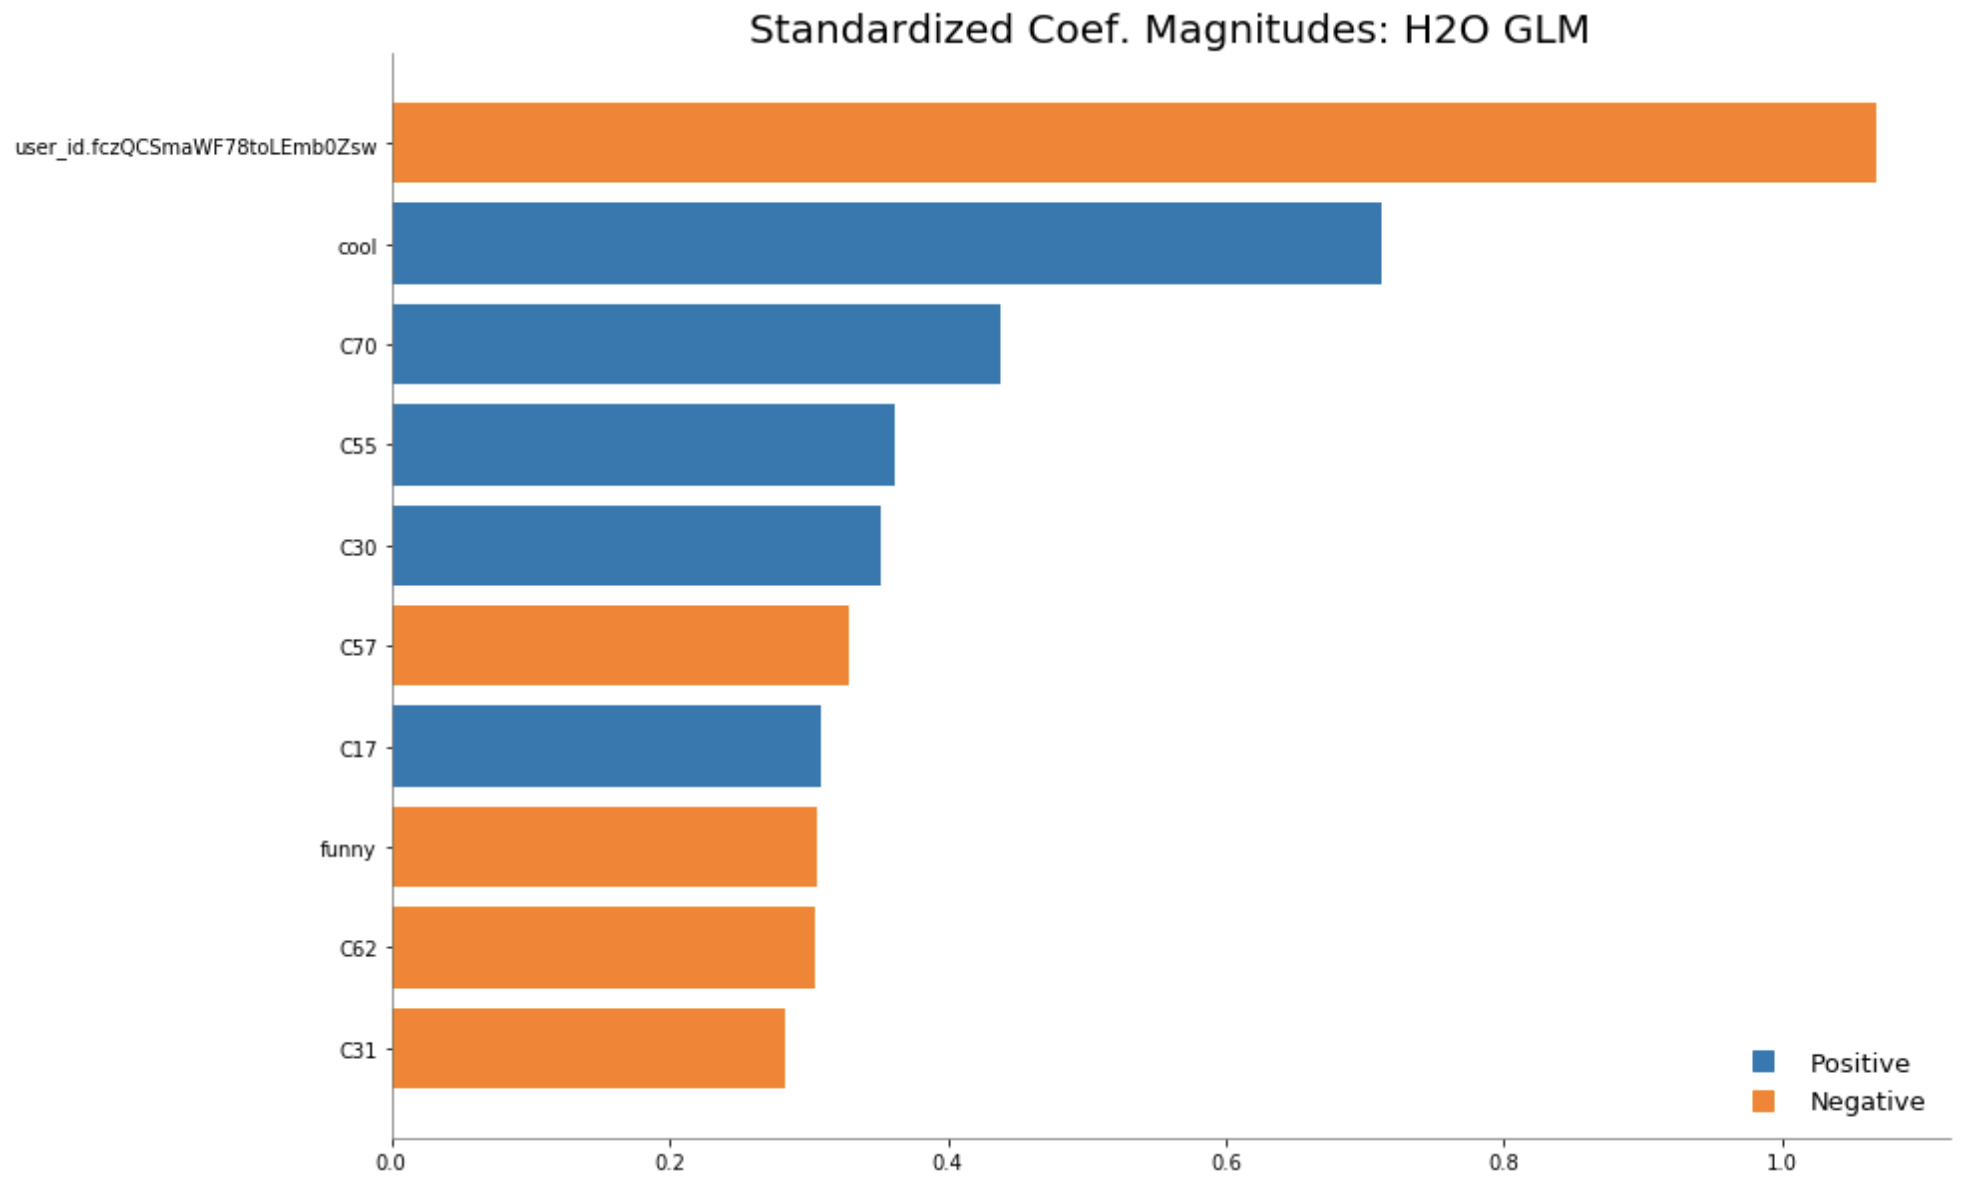
\includegraphics[width=6cm]{plots/yelp/y_vi_glm.png}
\end{minipage}
}
\subfigure[Logistic Regression]{
\begin{minipage}[t]{0.48\textwidth}
\centering
\label{Fig.y.v.2}
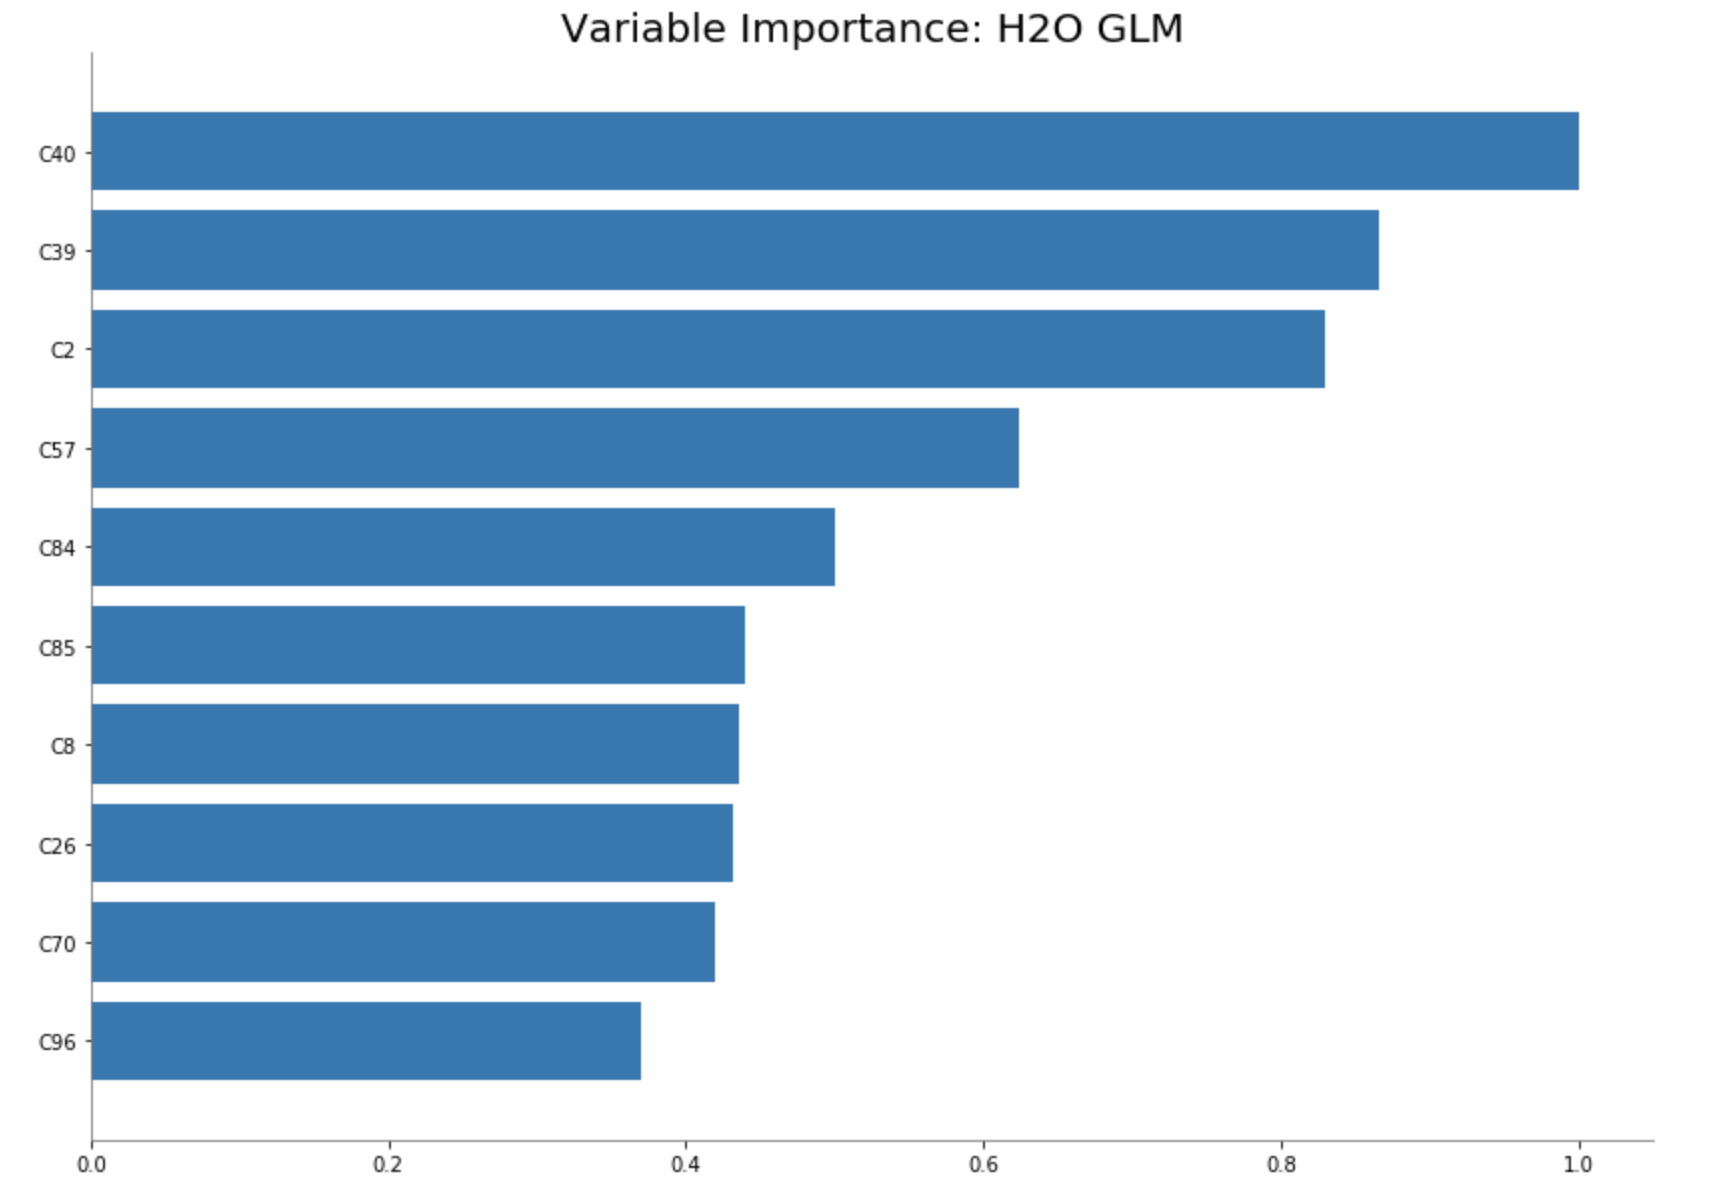
\includegraphics[width=6cm]{plots/yelp/y_vi_lr.png}
\end{minipage}
}
\quad
\subfigure[Gradient Boosting I]{
\begin{minipage}[t]{0.48\textwidth}
\centering
\label{Fig.y.v.3}
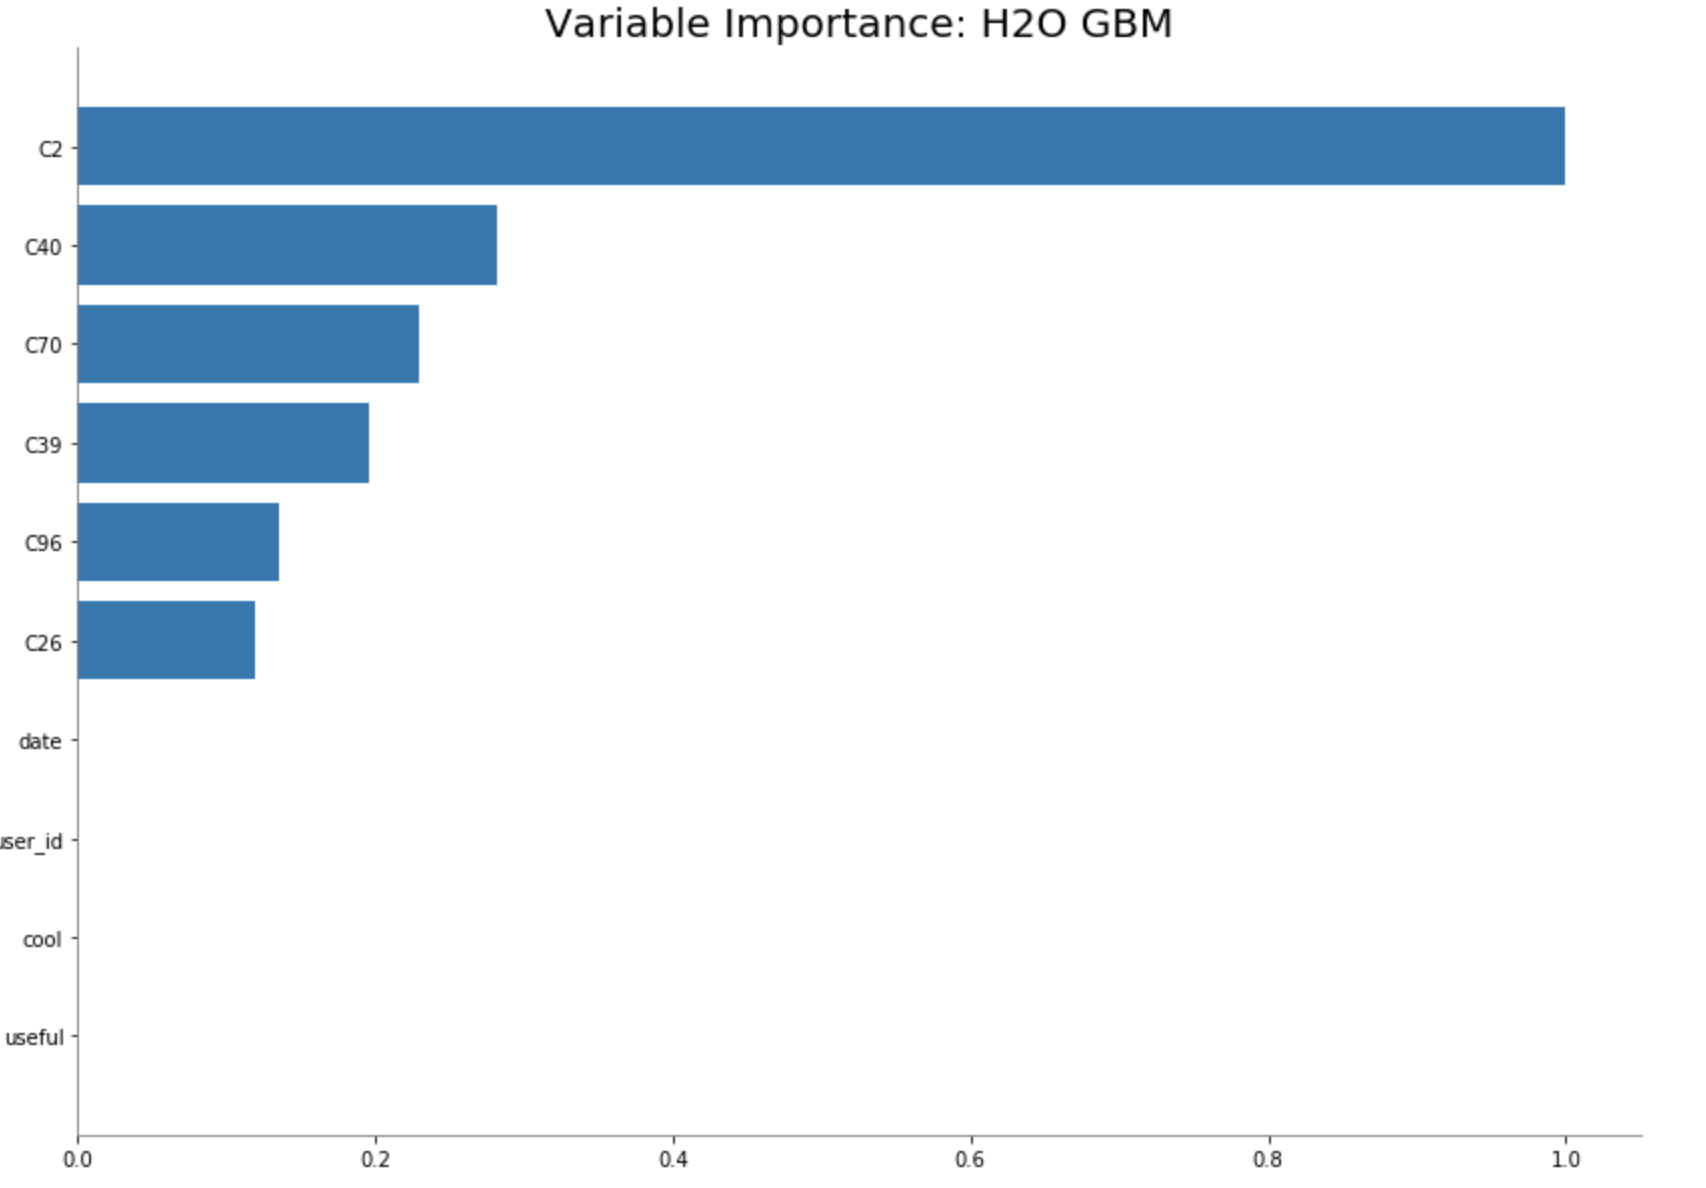
\includegraphics[width=6.1cm]{plots/yelp/y_vi_gbm1.png}
\end{minipage}
}
\subfigure[Gradient Boosting II]{
\begin{minipage}[t]{0.48\textwidth}
\centering
\label{Fig.y.v.4}
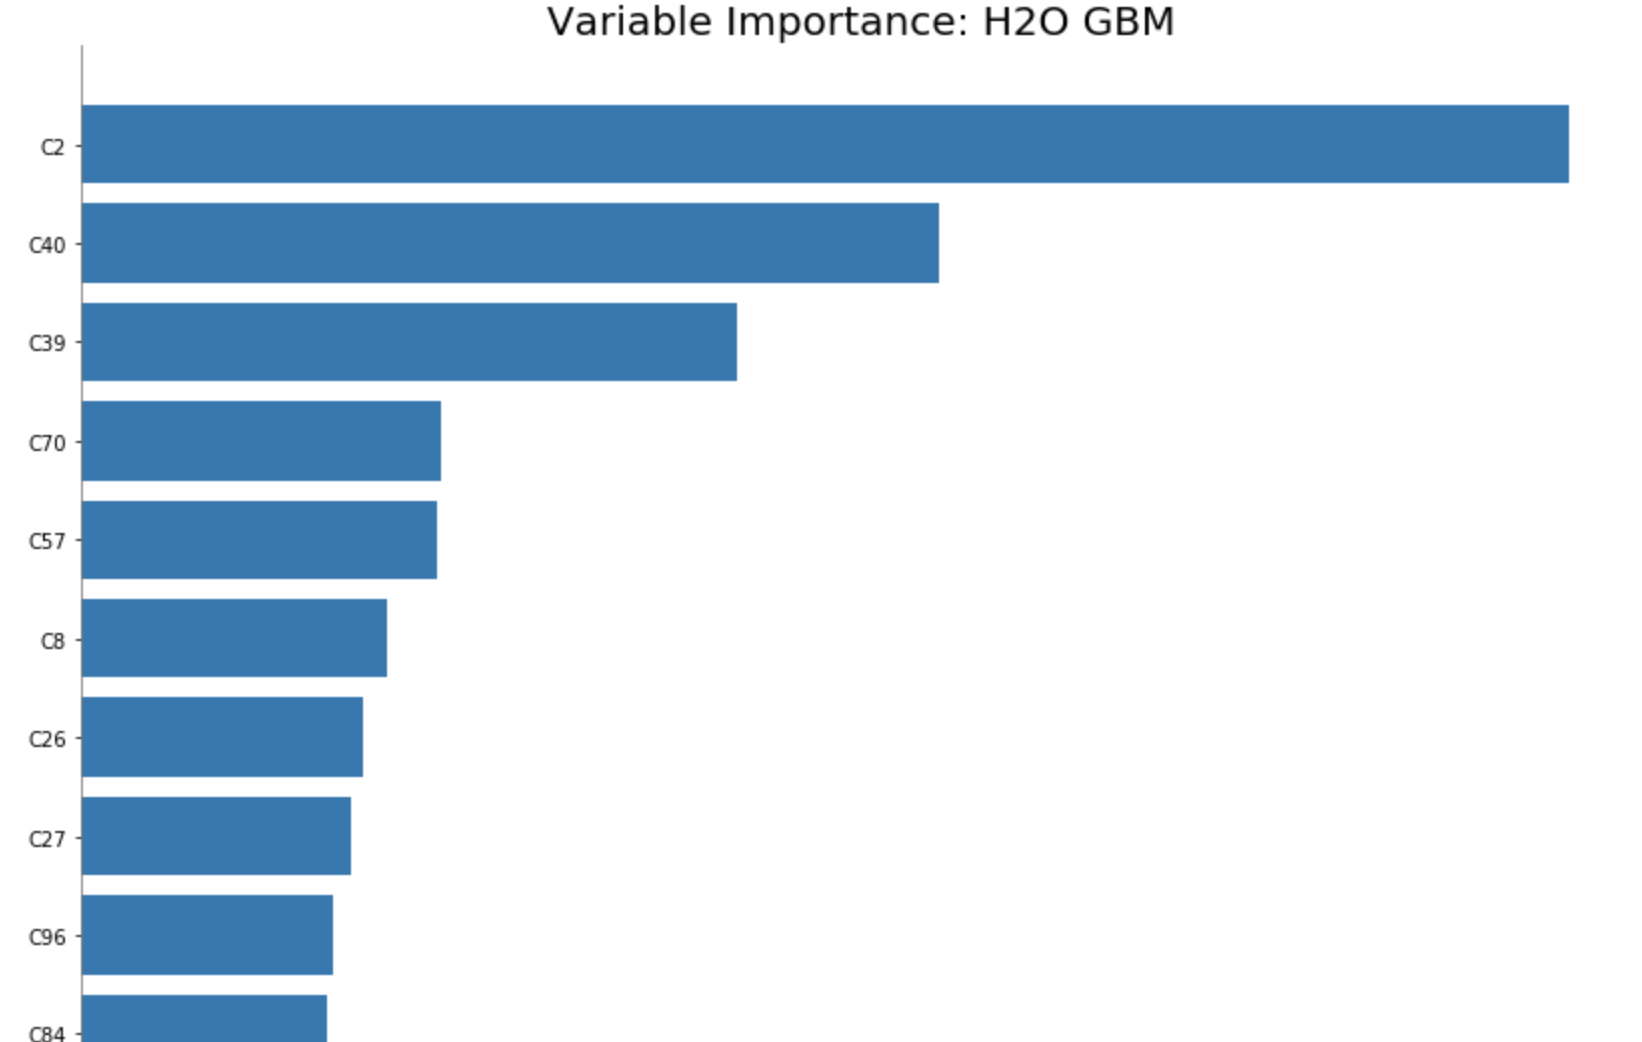
\includegraphics[width=6.3cm]{plots/yelp/y_vi_gbm2.png}
\end{minipage}
}
\caption{Variable Importance/ Standardized Coefficient Plots for Yelp Reviews}
\label{Fig.y.v}
\end{figure}

\subsubsection{Partial Dependence Plot}
Figure \ref{Fig.y.p} has four sub figures for different models' Partial Dependence Plots (PDP) in Yelp Review. We use the most important feature which we got in Figure \ref{Fig.y.v} as x axis, and the mean of response variables is the y axis. In Generalized Linear Model, We can get that the positive reviews always have a "cool" larger than 20, and in Logistic Regression, the larger the C40 is, the larger probability to get a positive review. In the last two Gradient Boosting Models, the mean of response variables change smoothly with the change of important feature C2.
\begin{figure}[H]
\centering
\subfigure[Generalized Linear]{
\begin{minipage}[t]{0.48\textwidth}
\centering
\label{Fig.y.p.1}
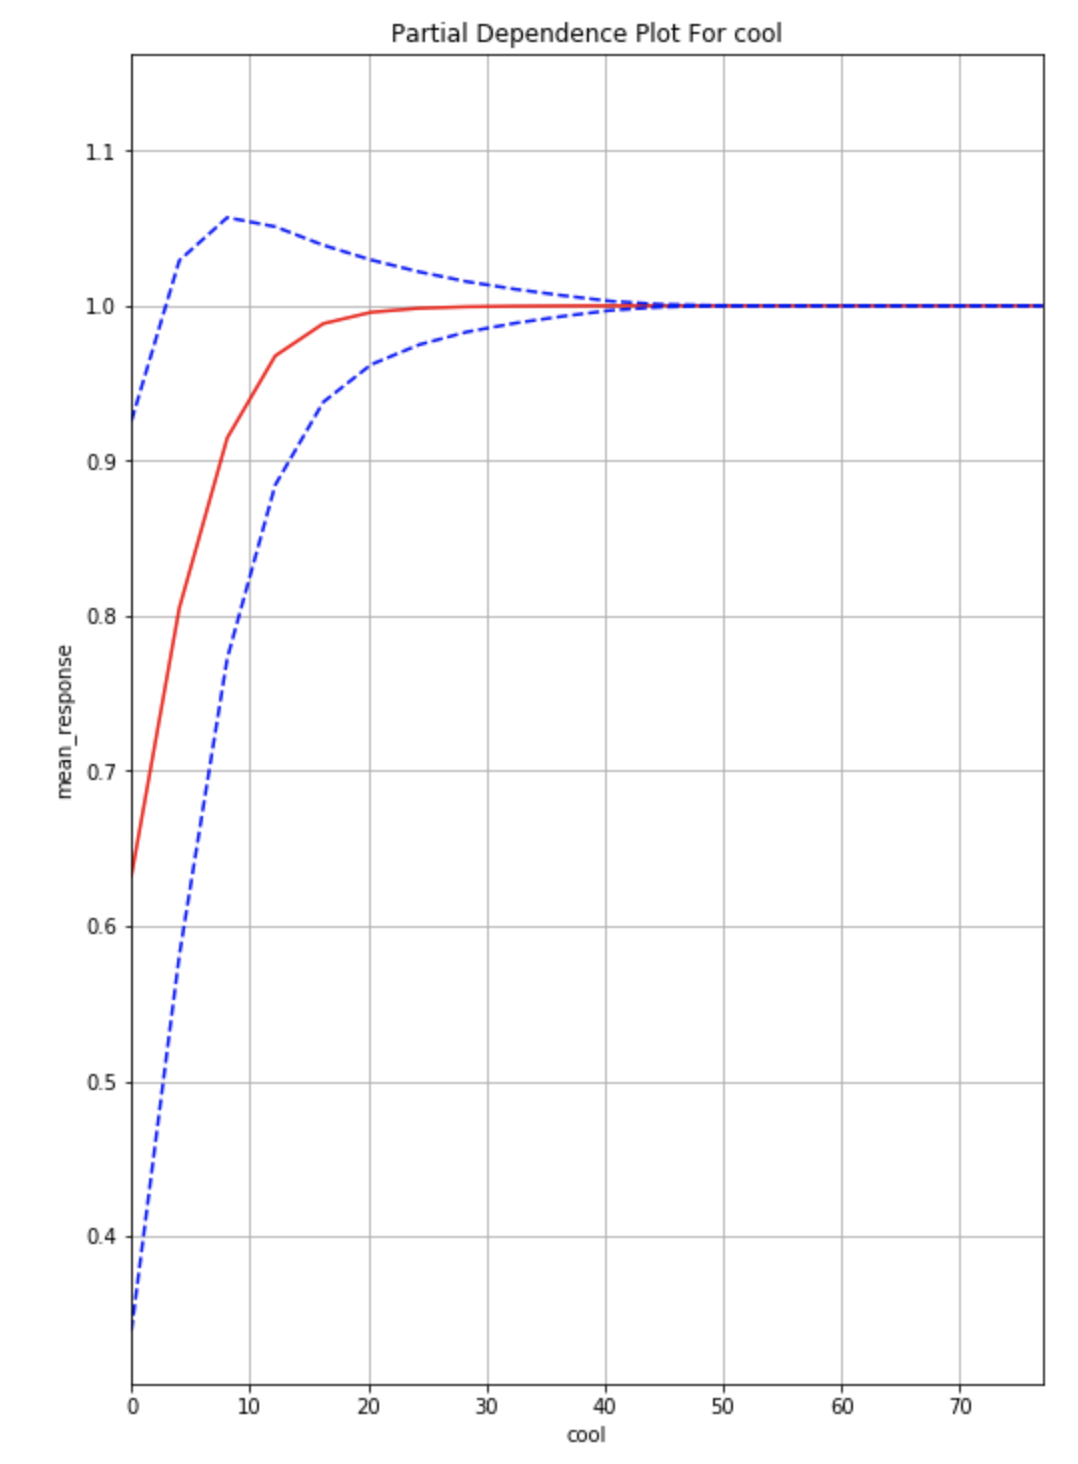
\includegraphics[width=6cm]{plots/yelp/y_pdp_glm.png}
\end{minipage}
}
\subfigure[Logistic Regression]{
\begin{minipage}[t]{0.48\textwidth}
\centering
\label{Fig.y.p.2}
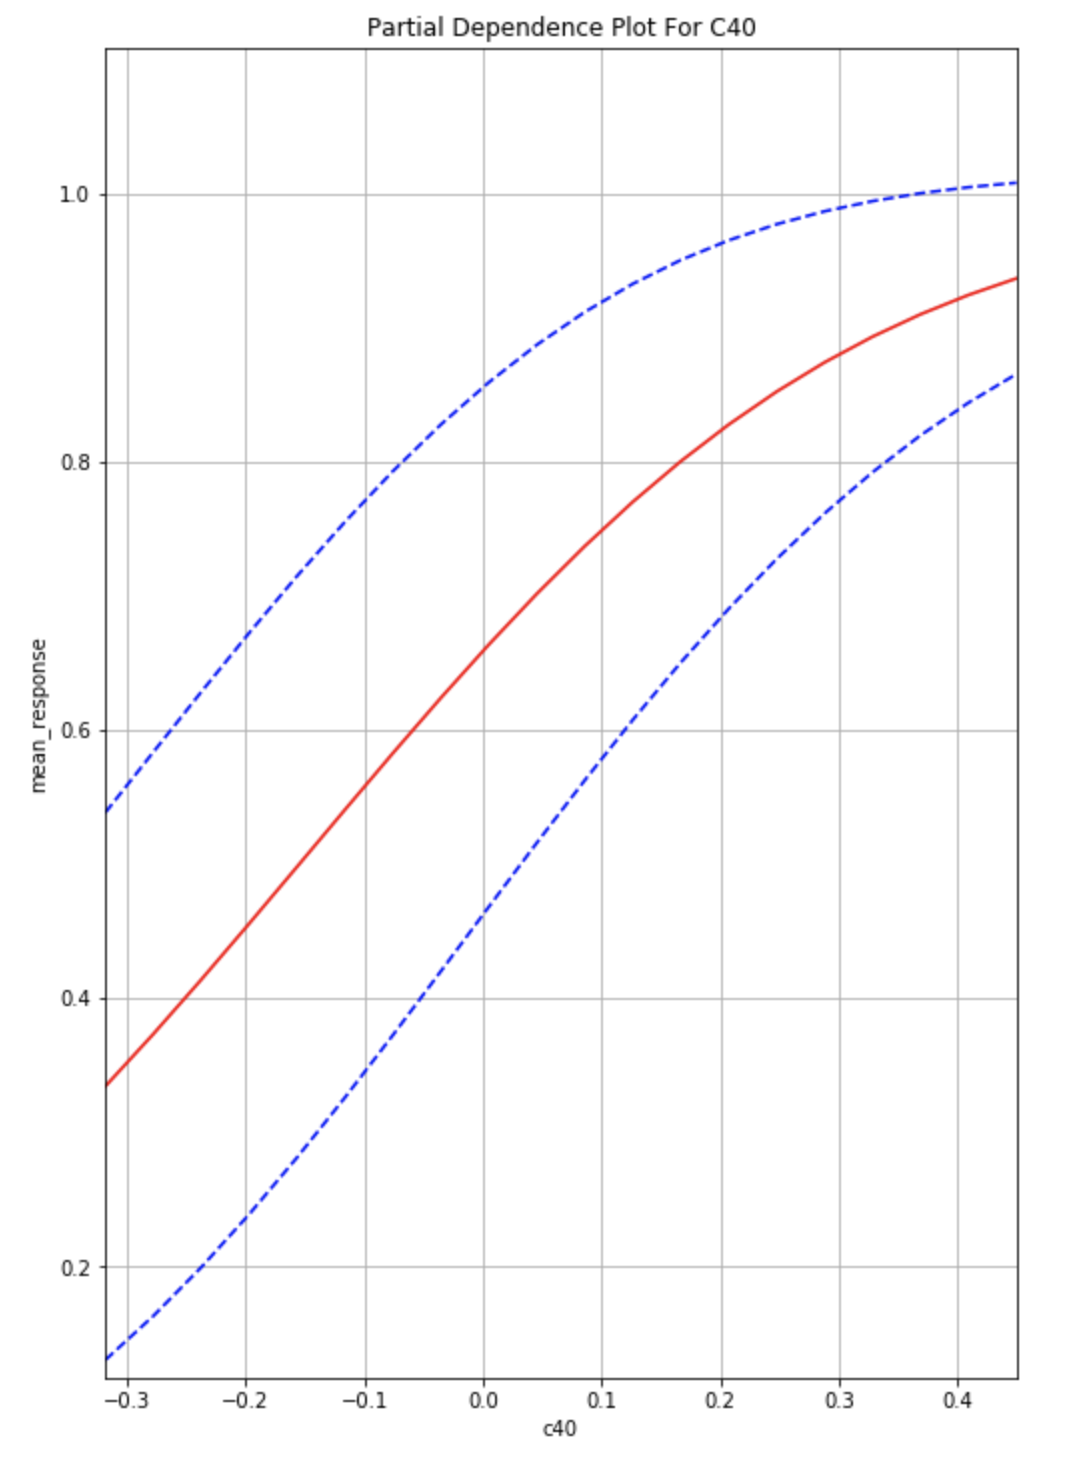
\includegraphics[width=6cm]{plots/yelp/y_pdp_lr.png}
\end{minipage}
}
\quad
\subfigure[Gradient Boosting I]{
\begin{minipage}[t]{0.48\textwidth}
\centering
\label{Fig.y.p.3}
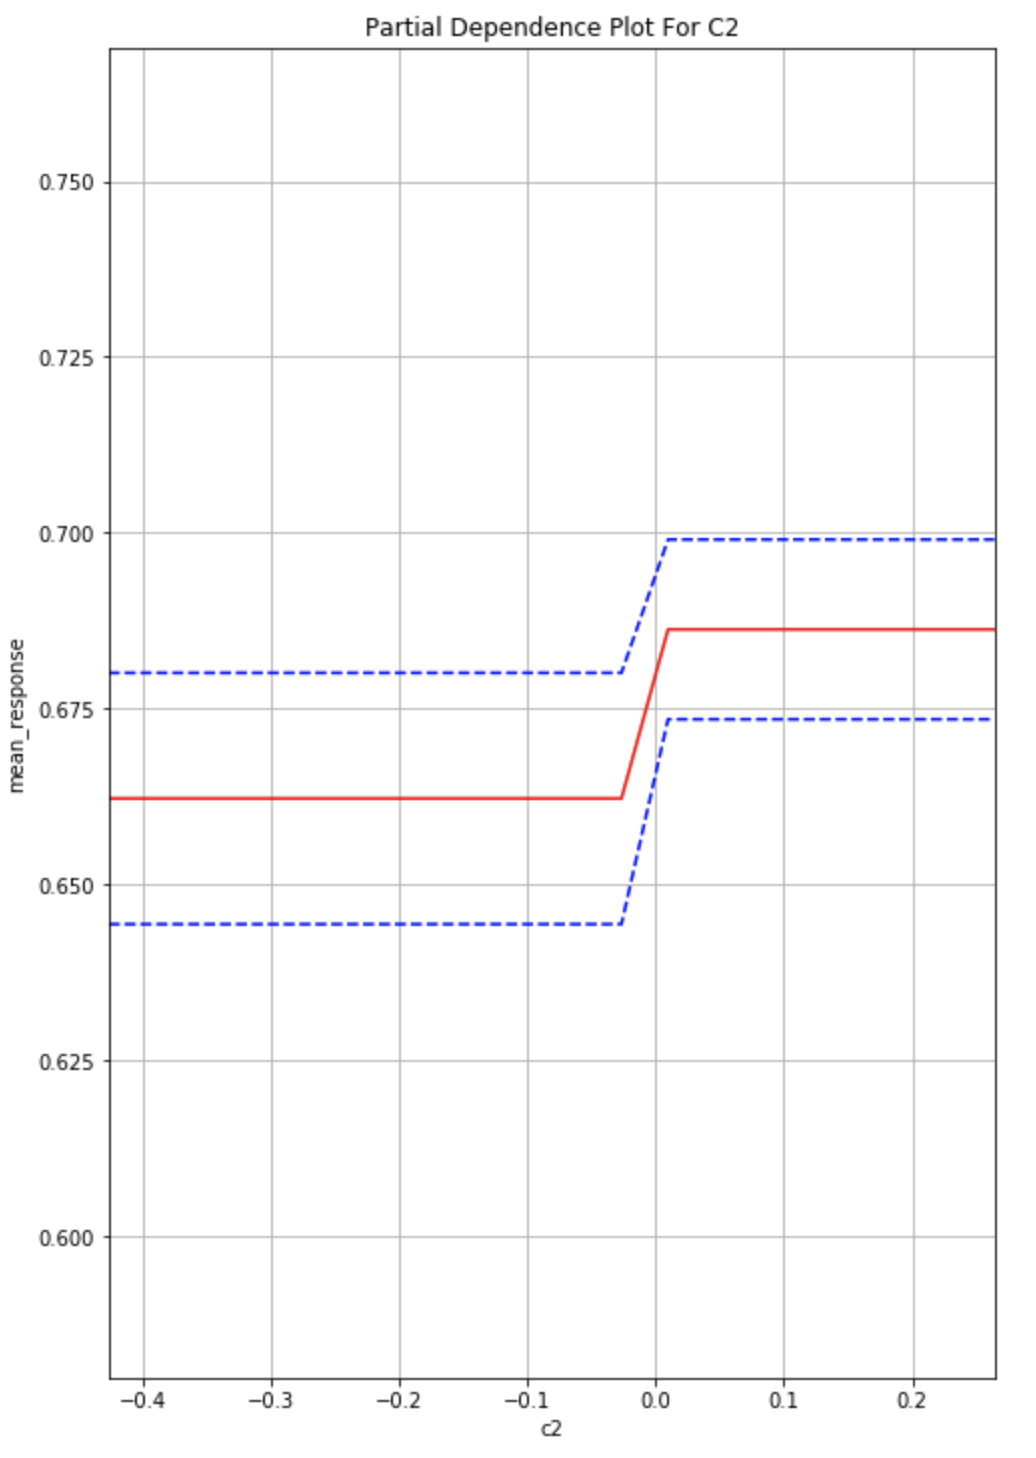
\includegraphics[width=6cm]{plots/yelp/y_pdp_gbm1.png}
\end{minipage}
}
\subfigure[Gradient Boosting II]{
\begin{minipage}[t]{0.48\textwidth}
\centering
\label{Fig.y.p.4}
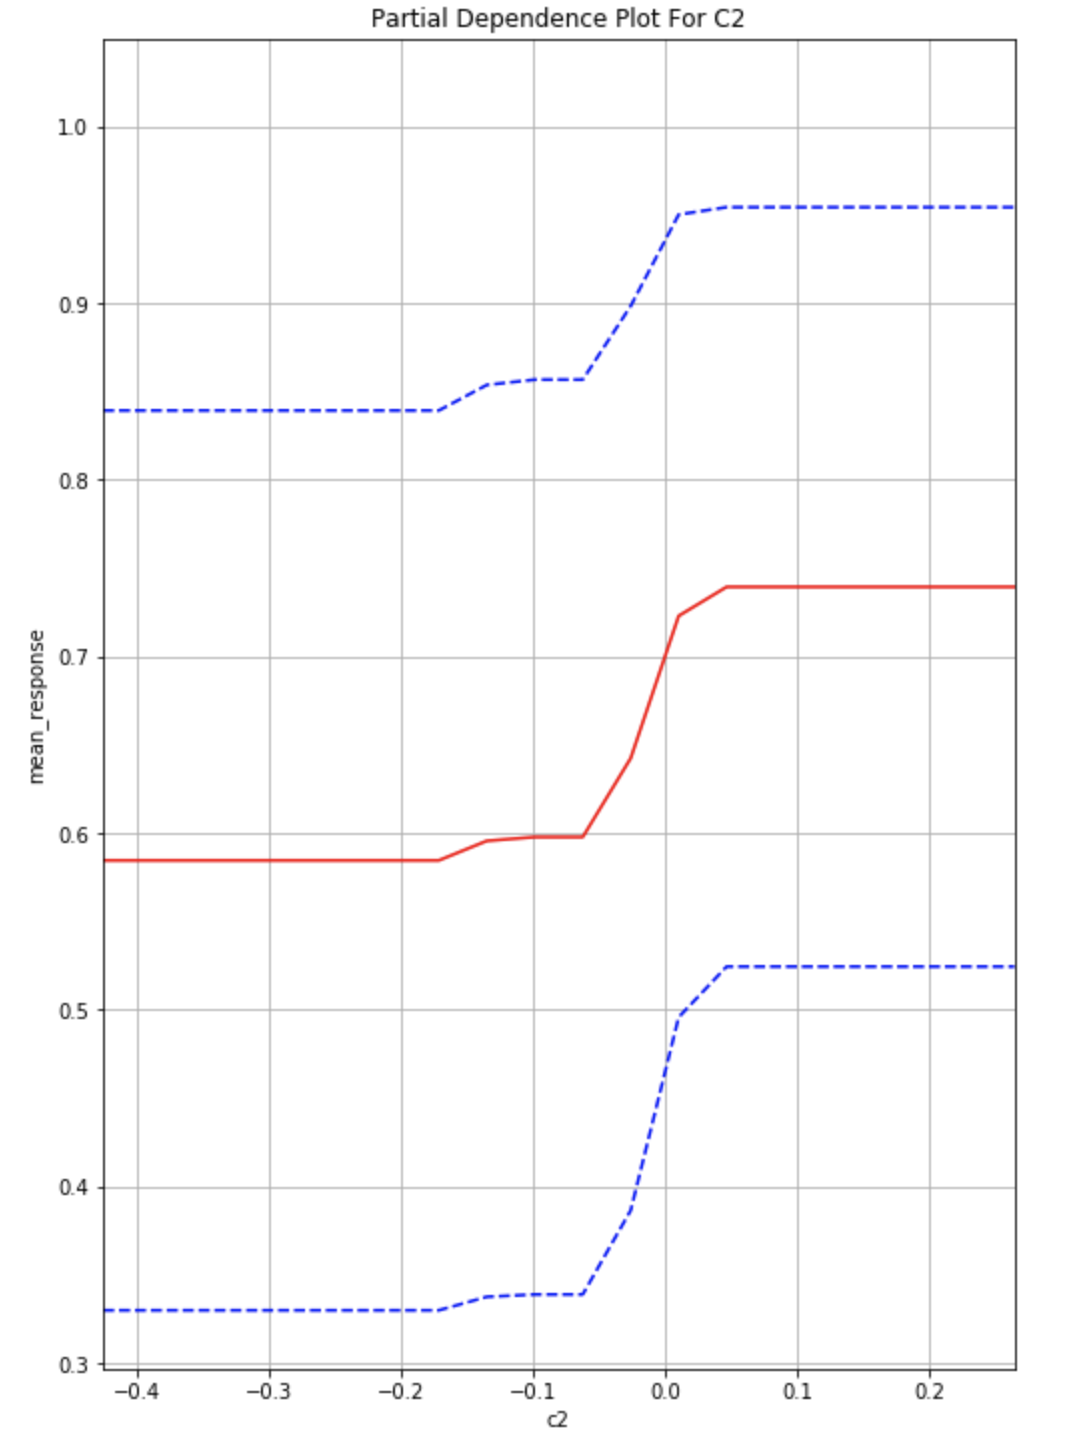
\includegraphics[width=6.2cm]{plots/yelp/y_pdp_gbm2.png}
\end{minipage}
}
\caption{Partial Dependence Plots (PDP) for Yelp Reviews}
\label{Fig.y.p}
\end{figure}

\subsubsection{Individual Conditional Expectation}
Figure \ref{Fig.y.i} has four sub figures for different models' Individual Conditional Expectation (ICE) in Yelp Review. We an get that the instances' distribution in each plot are similar to the Figure \ref{Fig.a.i} which are ICE for Amazon Review. on the other hand, we can also get the information between different instances in each model, for example the Figure \ref{Fig.y.i.2}, c40 is uniformly distributed, so the  the mean of the probability rises everywhere uniformly, but C2 in Figure \ref{Fig.y.i.4} it is opposite.

\begin{figure}[H]
\centering
\subfigure[Generalized Linear]{
\begin{minipage}[t]{0.48\textwidth}
\centering
\label{Fig.y.i.1}
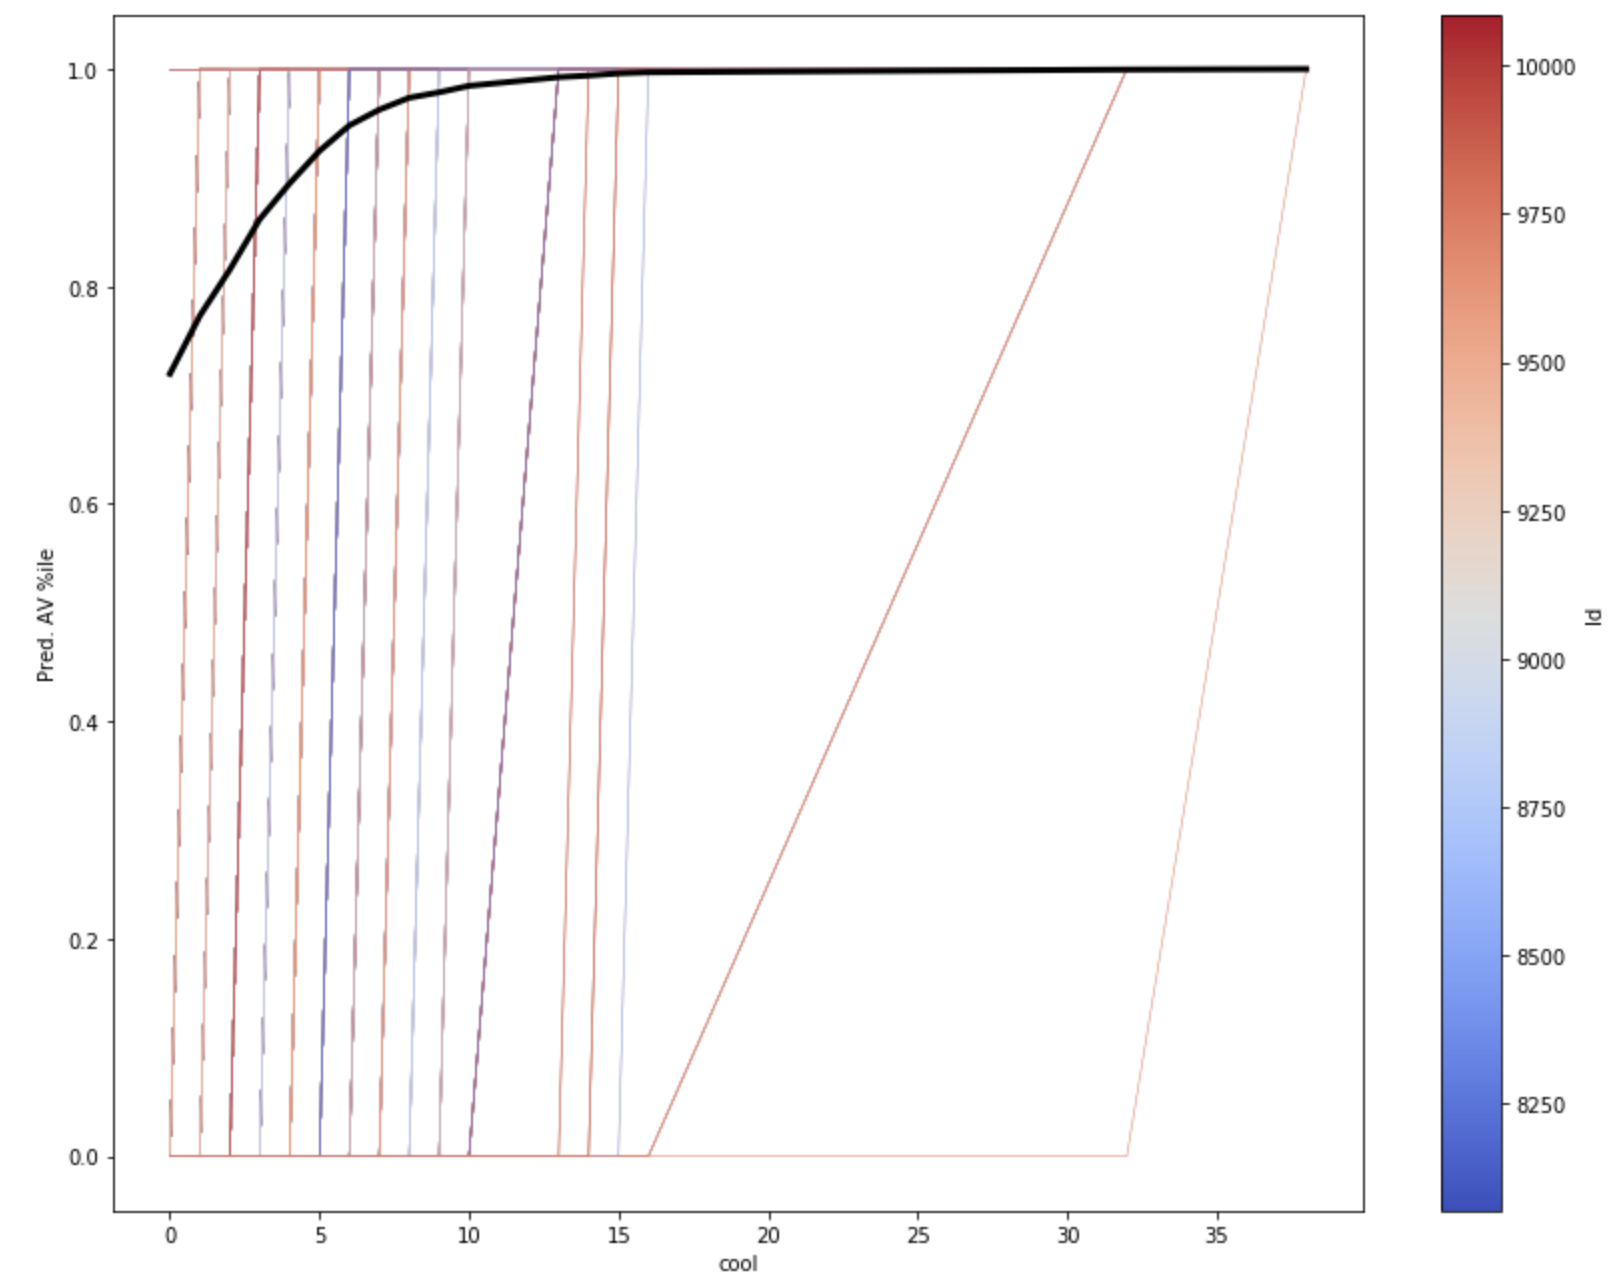
\includegraphics[width=6cm]{plots/yelp/y_ice_glm.png}
\end{minipage}
}
\subfigure[Logistic Regression]{
\begin{minipage}[t]{0.48\textwidth}
\centering
\label{Fig.y.i.2}
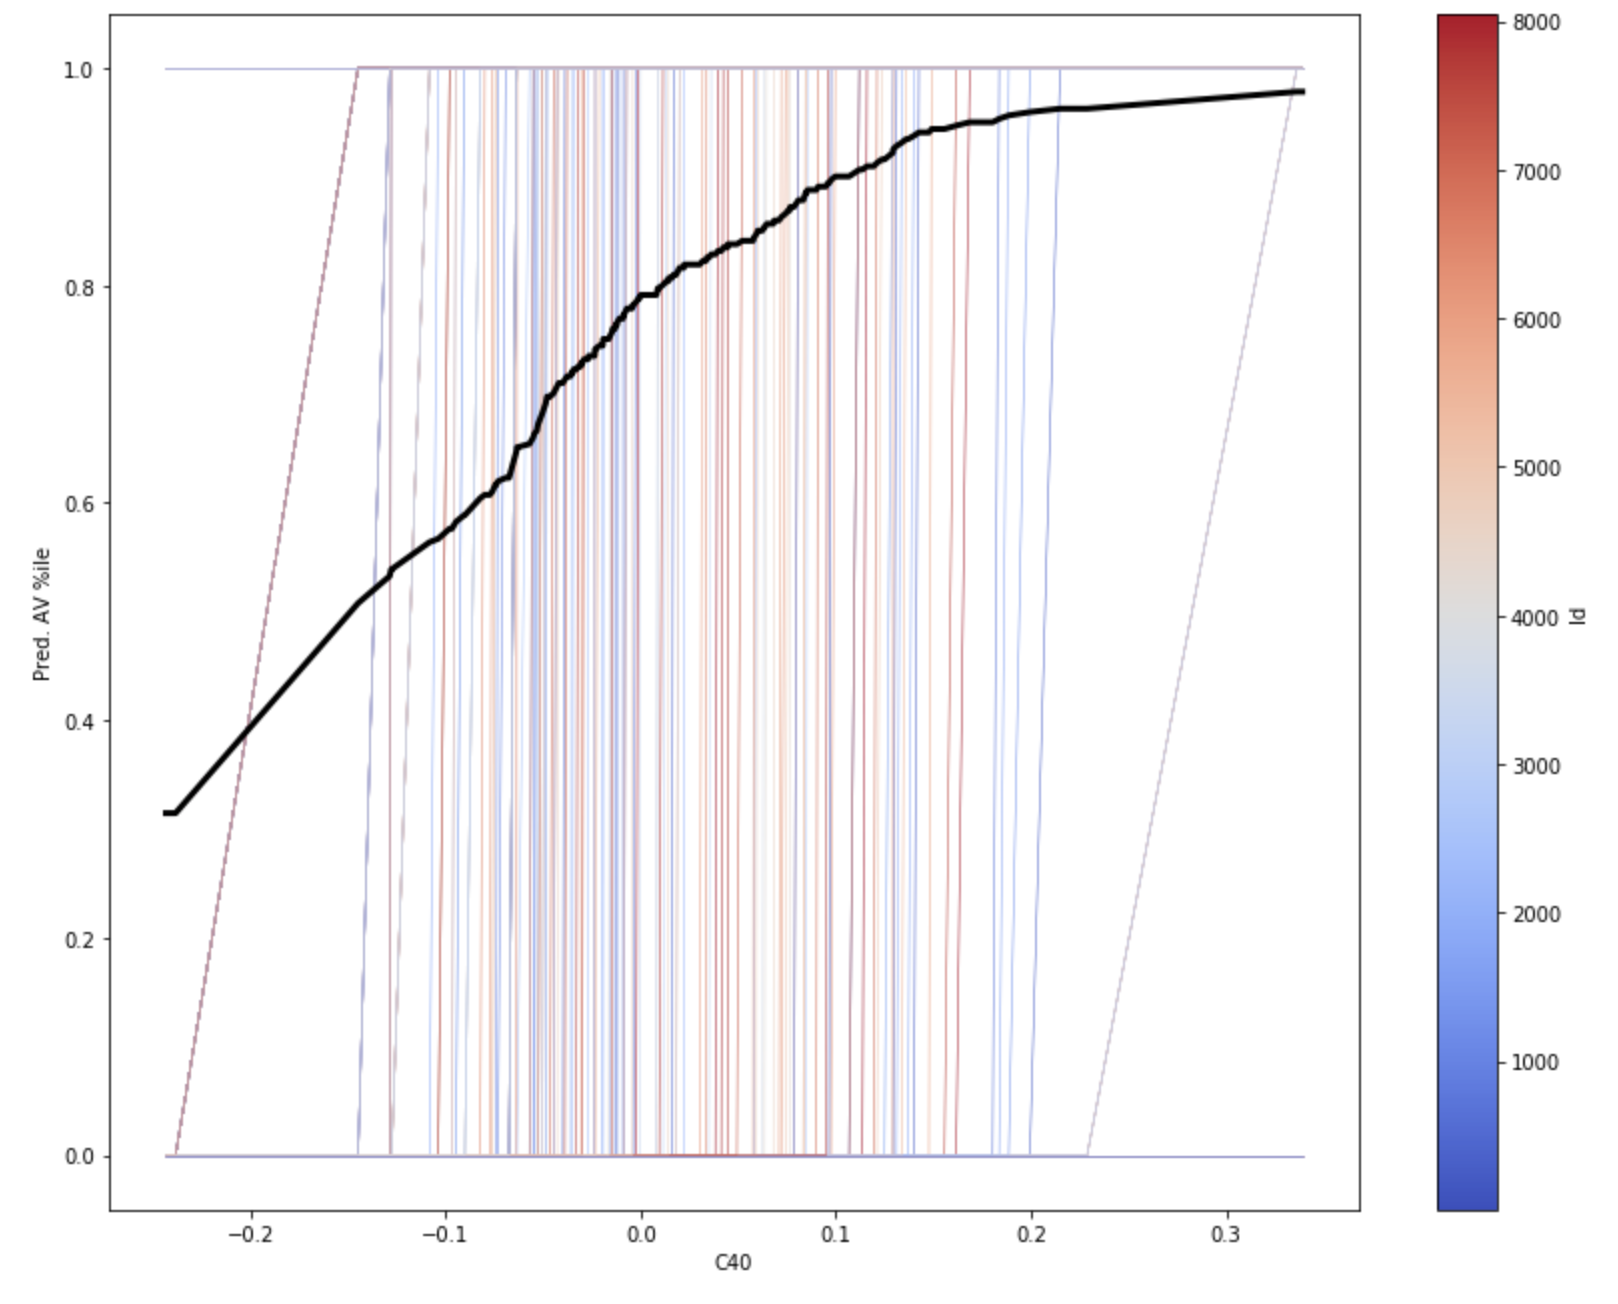
\includegraphics[width=6cm]{plots/yelp/y_ice_lr.png}
\end{minipage}
}
\quad
\subfigure[Gradient Boosting I]{
\begin{minipage}[t]{0.48\textwidth}
\centering
\label{Fig.y.i.3}
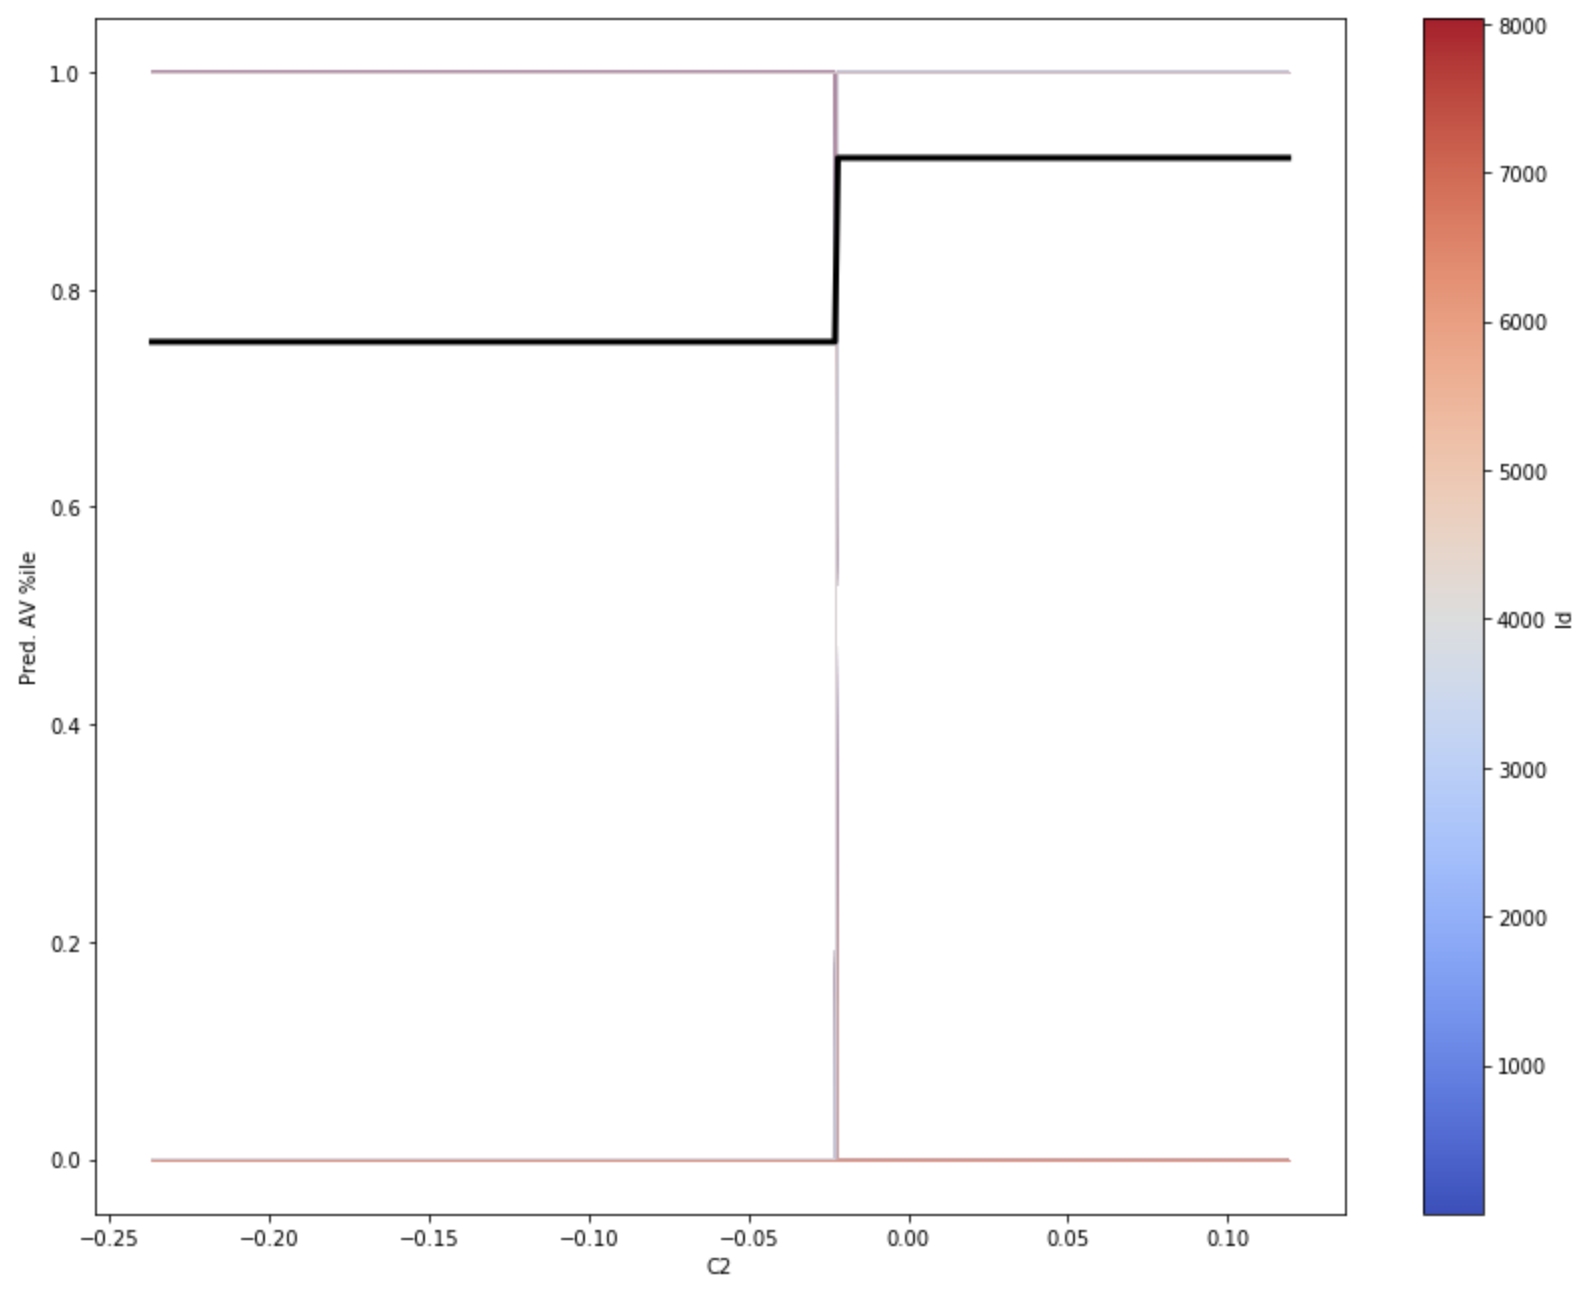
\includegraphics[width=6cm]{plots/yelp/y_ice_gbm1.png}
\end{minipage}
}
\subfigure[Gradient Boosting II]{
\begin{minipage}[t]{0.48\textwidth}
\centering
\label{Fig.y.i.4}
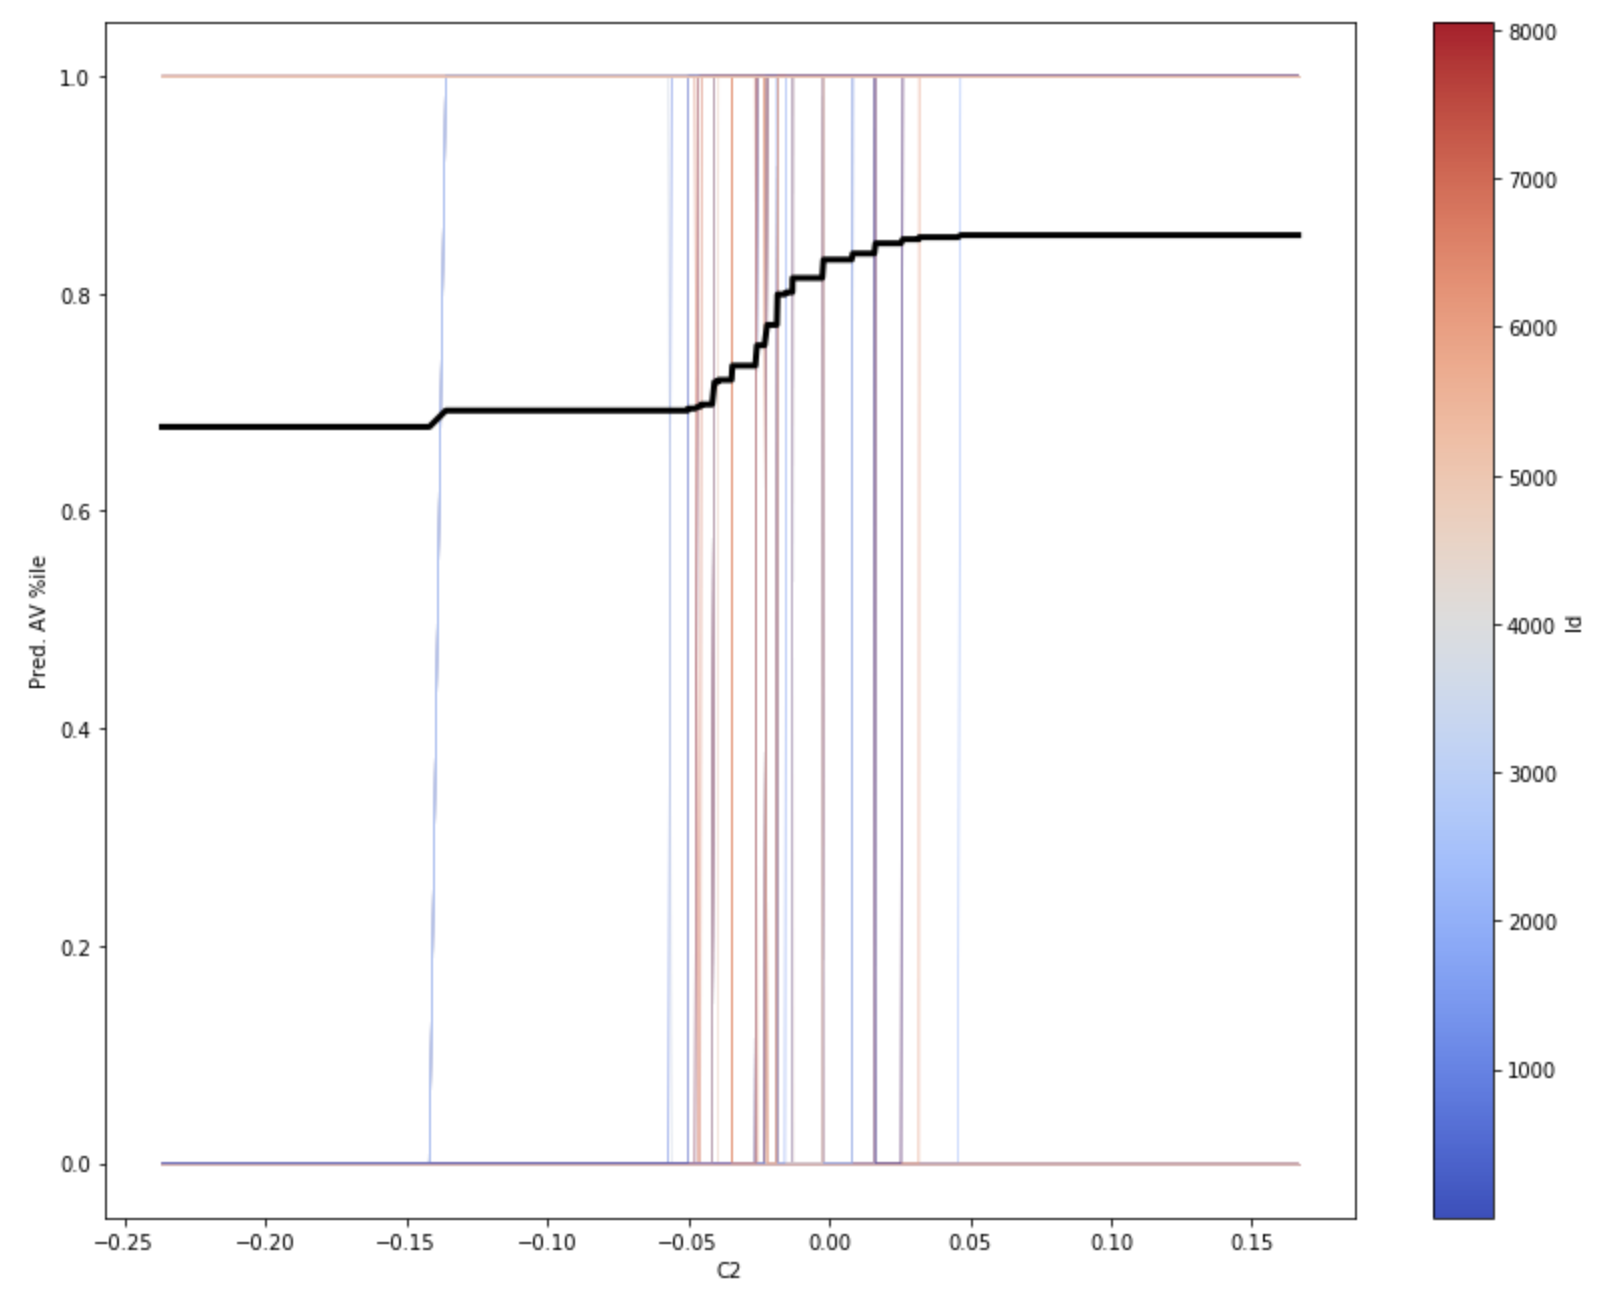
\includegraphics[width=6.2cm]{plots/yelp/y_ice_gbm2.png}
\end{minipage}
}
\caption{Individual Conditional Expectation (ICE) for Yelp Reviews}
\label{Fig.y.i}
\end{figure}


\section{Discussion}
As we can see the plots of prototype and new dataset in Result part, we can draw the conclusion that our interpretable prototype does well at least in review type of dataset, with the prove that we only slightly adjust the code to fit the new dataset and it still runs well. 

\subsection{Amazon (prototype)}
\subsubsection{Compare and Select the Best Model}
We can easily select the model which has the best performance based on matrix AUC score. In this case, Generalized Linear Model has the highest AUC score, which is 0.878. Thus, all interpretable explanation would be based on model Generalized Linear Model.
\subsubsection{Interpretability}
As for the GLM model, the importance of predictors can be detected by standard coefficients value. Thus, “HelpfulnessNumerator” has the highest absolute value of standard coefficients which means it is the most important predictor in this case.
It makes sense since in the real world, people intend to trust the comments when others willing to stand for. And from the partial dependence plot, we can draw the conclusion that people more likely to give a positive review when the number of Helpfulness is greater than 50.
In ICE plots, it’s obvious that the lower the review score, the higher the number of “HelpfulnessNumerator” needs in order to get a good review.


\subsection{Yelp (testing)}
\subsubsection{Compare and Select the Best Model}
With the help of tables of AUC score, we are able to select the best model for the Yelp Reviews dataset, that is Generalized Linear Model. The AUC of GBM is 0.876, and the three interpretable plots for this model will be the one we choose to further explain. 

\subsubsection{Interpretability}
As we can see from the standardized coefficient plot, predictor “user\_id” take the lead. We can understand this circumstance as some people willing to give average high score while others has a strict standards for the items they grade.
From the partial dependence plot of predictor “cool”, we can conclude that the number of “cool” is making huge different when range 0 to 20. However, once the number of “cool” excess 20, it won’t be that important for the score of reviews.
With the help of ICE plots, we find out that most of the “cool” number is range from 0 to 15 and evenly distributed.


\subsection{Future}
\begin{itemize}
\item For the prototype, we will enrich our model interpretability. In order to make our interpretability more easily and clearly, we plan to use pandas library to generate LIME, ALE and other interpretable plots. 

\item For testing data, since all the data we interpret so far is Reviews data. In the future, we will try some different types of dataset and try to improve our prototype also fit these types of dataset.

\item In addition, we also need to create a user interface for customers. From this interface, customers only need to provide limit predictors like original dataset and would be able to obtain the interpretable plots and explanations as well.

\item We used text formatting datasets in final project, in the future, we will add image samples to make our model suit for more situations.

\end{itemize}

\bibliographystyle{unsrt}  
%\bibliography{references}  %%% Remove comment to use the external .bib file (using bibtex).
%%% and comment out the ``thebibliography'' section.


%%% Comment out this section when you \bibliography{references} is enabled.
\begin{thebibliography}{1}

\bibitem{glm}
\newblock Generalized Linear Models and Mixed-Effects in Agriculture.
\url{https://www.r-bloggers.com/generalized-linear-models-and-mixed-effects-in-agriculture/}

\bibitem{ml}
\newblock Machine Learning for Particle Data When You are Not a Physicist.
\url{https://towardsdatascience.com/machine-learning-for-particle-data-when-you-are-not-a-physicist-dad77beb90e0}

\bibitem{statistics}
Pratap Dangeti .
\newblock  In {\em Statistics for Machine Learning}, July 2017.

\bibitem{christoph}
Christoph Molnar.
\newblock Fast classification of handwritten on-line arabic characters.
\newblock In {\em Interpretable Machine Learning}, April 2019.

\bibitem{plot}
\newblock Interpretable Machine Learning with Python.
\url{https://github.com/jphall663/interpretable_machine_learning_with_python}
% \bibitem{christoph2}
% Christoph Molnar.
% \newblock Fast classification of handwritten on-line arabic characters.
% \newblock In {\em Interpretable Machine Learning}, April 2019.

\bibitem{AutoML}
H2O AutoML.
\newblock Automatic Machine Learning.
\url{http://docs.h2o.ai/h2o/latest-stable/h2o-docs/automl.html#automl-automatic-machine-learning}

\bibitem{pdp}
Friedman, Jerome H
\newblock Greedy function approximation: A gradient boosting machine.
\newblock In {\em Annals of statistics}, 2001: 1189-1232.

\end{thebibliography}

\pagebreak 

\appendix
\section{} 
\label{sec:App}
\lstset{
    language=python,
    numbers=left, 
    numberstyle= \tiny, 
    keywordstyle= \color{ blue!70},
    commentstyle= \color{red!50!green!50!blue!50}, 
    frame=shadowbox, 
    rulesepcolor= \color{ red!20!green!20!blue!20} ,
    escapeinside=``, 
    xleftmargin=1em,xrightmargin=0em, aboveskip=1em,
    framexleftmargin=2em
} 
\begin{lstlisting}
from __future__ import division

import six

from matplotlib import colors, cm
from matplotlib import pyplot as plt
import numpy as np
import pandas as pd
import h2o

def _get_grid_points(x, num_grid_points):
    if num_grid_points is None:
        return x.unique()
    else:
        # unique is necessary, because if num_grid_points is too much 
        # larger than x.shape[0], there will be duplicate quantiles (even 
        # with interpolation)
        return x.quantile(np.linspace(0, 1, num_grid_points)).unique()


def _get_point_x_ilocs(grid_index, data_index):
    data_level = 'data_{}'.format(grid_index.name)

    return (np.abs(np.subtract
                      .outer(grid_index,
                             data_index.get_level_values(data_level)))
              .argmin(axis=0))


def _get_quantiles(x):
    return np.greater.outer(x, x).sum(axis=1) / x.size


def ice(data, column, model, num_grid_points=None):
    """
    Generate individual conditional expectation (ICE) curves for a model.

    :param data: the sample data from which to generate ICE curves
    :type data: ``pandas`` ``DataFrame``

    :param column: the name of the column in ``data`` that will be varied to
        generate ICE curves
    :type column: ``str``

    :param predict: the function that generates predictions from the model.
        Must accept a ``DataFrame`` with the same columns as ``data``.
    :type predict: callable

    :param num_grid_points: the number of grid points to use for the 
        independent variable of the ICE curves. The independent variable 
        values for the curves will be quantiles of the data.

        If ``None``, the values of the independent variable will be the unique
        values of ``data[column]``.
    :type num_grid_points: ``None`` or ``int``

    :return: A ``DataFrame`` whose columns are ICE curves.  The row index is the
        independent variable, and the column index is the original data point
        corresponding to that ICE curve.
    :rtype: ``pandas`` ``DataFrame``
    """
    data = data.as_data_frame()
    x_s = _get_grid_points(data[column], num_grid_points)
    ice_data, orig_column = _to_ice_data(data, column, x_s)
    hf = h2o.H2OFrame(ice_data)
    hfd = model.predict(hf)
    ice_data['ice_y'] = hfd.as_data_frame()['predict'].as_matrix()
    ice_data['data_{}'.format(column)] = orig_column

    other_columns = ['data_{}'.format(column)] + 
             [col for col in data.columns if col != column]
    ice_data = ice_data.pivot_table(values='ice_y', 
             index=other_columns, columns=column).T

    return ice_data


def ice_plot(ice_data, frac_to_plot=1.,
             plot_points=False, point_kwargs=None,
             x_quantile=False, plot_pdp=False,
             centered=False, centered_quantile=0.,
             color_by=None, cmap=None, figsize=(14,11),
             ax=None, pdp_kwargs=None, **kwargs):
    """
    Plot the ICE curves

    :param ice_data: the ICE data generated by :func:`pycebox.ice.ice`
    :type ice_data: ``pandas`` ``DataFrame``

    :param frac_to_plot: the fraction of ICE curves to plot. If less than 
        one, randomly samples columns of ``ice_data`` to plot.
    :type frac_to_plot: ``float``

    :param plot_points: whether or not to plot the original data points on
        the ICE curves.  In this case, ``point_kwargs`` is passed as keyword
        arguments to plot.
    :type plot_points: ``bool``

    :param x_quantile: if ``True``, the plotted x-coordinates are the quantiles 
    of ``ice_data.index``
    :type x_quantile: ``bool``

    :param plot_pdp: if ``True``, plot the partial depdendence plot.  In this
        case, ``pdp_kwargs`` is passed as keyword arguments to ``plot``.

    :param centered: if ``True``, each ICE curve is centered to zero at the
        percentile closest to ``centered_quantile``.
    :type centered: ``bool``

    :param color_by:  If a string, color the ICE curve by that level of the
        column index.

        If callable, color the ICE curve by its return value when applied to 
        a ``DataFrame`` of the column index of ``ice_data``
    :type color_by: ``None``, ``str``, or callable

    :param cmap:
    :type cmap: ``matplotlib`` ``Colormap``

    :param figsize: size of the figure
    :type figsize: tuple (width, height)
        
    :param ax: the ``Axes`` on which to plot the ICE curves
    :type ax: ``None`` or ``matplotlib`` ``Axes``

    Other keyword arguments are passed to ``plot``
    """
    if not ice_data.index.is_monotonic_increasing:
        ice_data = ice_data.sort_index()

    if centered:
        quantiles = _get_quantiles(ice_data.index)
        centered_quantile_iloc = np.abs(quantiles - centered_quantile)
              .argmin()
        ice_data = ice_data - ice_data.iloc[centered_quantile_iloc]

    if frac_to_plot < 1.:
        n_cols = ice_data.shape[1]
        icols = np.random.choice(n_cols, size=frac_to_plot * n_cols, 
              replace=False)
        plot_ice_data = ice_data.iloc[:, icols]
    else:
        plot_ice_data = ice_data


    if x_quantile:
        x = _get_quantiles(ice_data.index)
    else:
        x = ice_data.index

    if plot_points:
        point_x_ilocs = _get_point_x_ilocs(plot_ice_data.index, 
               plot_ice_data.columns)
        point_x = x[point_x_ilocs]
        point_y = plot_ice_data.values[point_x_ilocs, 
               np.arange(point_x_ilocs.size)]

        
    if ax is None:
        _, ax = plt.subplots(figsize=figsize)

    if color_by is not None:
        if isinstance(color_by, six.string_types):
            colors_raw = plot_ice_data.columns.get_level_values(color_by)
                   .values
        elif hasattr(color_by, '__call__'):
            col_df = pd.DataFrame(list(plot_ice_data.columns.values),
            columns=plot_ice_data.columns.names)
            colors_raw = color_by(col_df)
        else:
            raise ValueError('color_by must be a string or function')

        norm = colors.Normalize(colors_raw.min(), colors_raw.max())
        m = cm.ScalarMappable(norm=norm, cmap=cmap)

        for color_raw, (_, ice_curve) in zip(colors_raw, 
                   plot_ice_data.iteritems()):
            c = m.to_rgba(color_raw)
            ax.plot(x, ice_curve, c=c, zorder=0, **kwargs)
    else:
        ax.plot(x, plot_ice_data, zorder=0, **kwargs)

    if plot_points:
        ax.scatter(point_x, point_y, zorder=10, **(point_kwargs or {}))

    if plot_pdp:
        pdp_kwargs = pdp_kwargs or {}
        pdp_data = pdp(ice_data)
        ax.plot(x, pdp_data, **pdp_kwargs)

    return ax


def pdp(ice_data):
    """
    Calculate a partial dependence plot from ICE data

    :param ice_data: the ICE data generated by :func:`pycebox.ice.ice`
    :type ice_data: ``pandas`` ``DataFrame``

    :return: the partial dependence plot curve
    :rtype: ``pandas`` ``Series``
    """
    return ice_data.mean(axis=1)


def _to_ice_data(data, column, x_s):
    """
    Create the DataFrame necessary for ICE calculations
    """
    ice_data = pd.DataFrame(np.repeat(data.values, x_s.size, axis=0), 
            columns=data.columns)
    data_column = ice_data[column].copy()
    ice_data[column] = np.tile(x_s, data.shape[0])

    return ice_data, data_column
\end{lstlisting}

\end{document}
